\documentclass[11pt,letterpaper]{article}
\usepackage[T1]{fontenc}\usepackage[utf8]{inputenc}
\usepackage[margin=1in]{geometry}\usepackage{graphicx,caption,float,pdflscape,booktabs,array,amsmath,amssymb,microtype}
\usepackage{xurl}\usepackage[hidelinks]{hyperref}
\usepackage[super,sort&compress]{natbib}
\providecommand{\bibcommenthead}{}
\graphicspath{{figures/}}\raggedright\raggedbottom\emergencystretch=3em
\newcolumntype{L}[1]{>{\raggedright\arraybackslash}p{#1}}
\newcommand{\gene}[1]{\textit{#1}}\setlength{\parskip}{0.4em}
\captionsetup{font=small,justification=raggedright,singlelinecheck=false}
\renewcommand{\tablename}{Supplementary Table}
\title{Supplementary Information\\[0.5em]\large Structure-Guided Proteogenomics Identifies ARID1A-Associated cBAF Protein Co-variation in Lung Cancer}
\author{\small Zhiyong Tao\textsuperscript{\textdagger}, Juan Xiong\textsuperscript{\textdagger}, Yiwei Zhang\textsuperscript{\textdagger}, Chulin Zhong\\\small Wenkai Gao, Guohua Fan, Yabing Huang\textsuperscript{*}}
\renewcommand{\thepage}{S\arabic{page}}
\date{}\begin{document}\maketitle
\begin{center}\small Department of Pathology, Renmin Hospital of Wuhan University,\\Wuhan 430060, China\\\textsuperscript{*}Correspondence: \href{mailto:ybhuang@whu.edu.cn}{ybhuang@whu.edu.cn}\\\textsuperscript{\textdagger}These authors contributed equally.\\[0.5em]Funding: General Program of the National Natural Science Foundation of China\\(Grant No. 62572360).\end{center}
\noindent\textbf{Supplementary Information.} This file contains Supplementary Figures S1--S20, Tables S1--S7, and extended methods and validation results. Underlying analysis files accompany Supplementary Data S1--S8. Figures S15--S19 preserve broader analyses removed from the focused main narrative; Figure S20 provides a descriptive replot of published molecular rescue data. Exploratory analyses are distinguished from the primary fixed-panel analyses.

\clearpage
\section*{Supplementary Figure S1}
\begin{figure}[H]
\centering
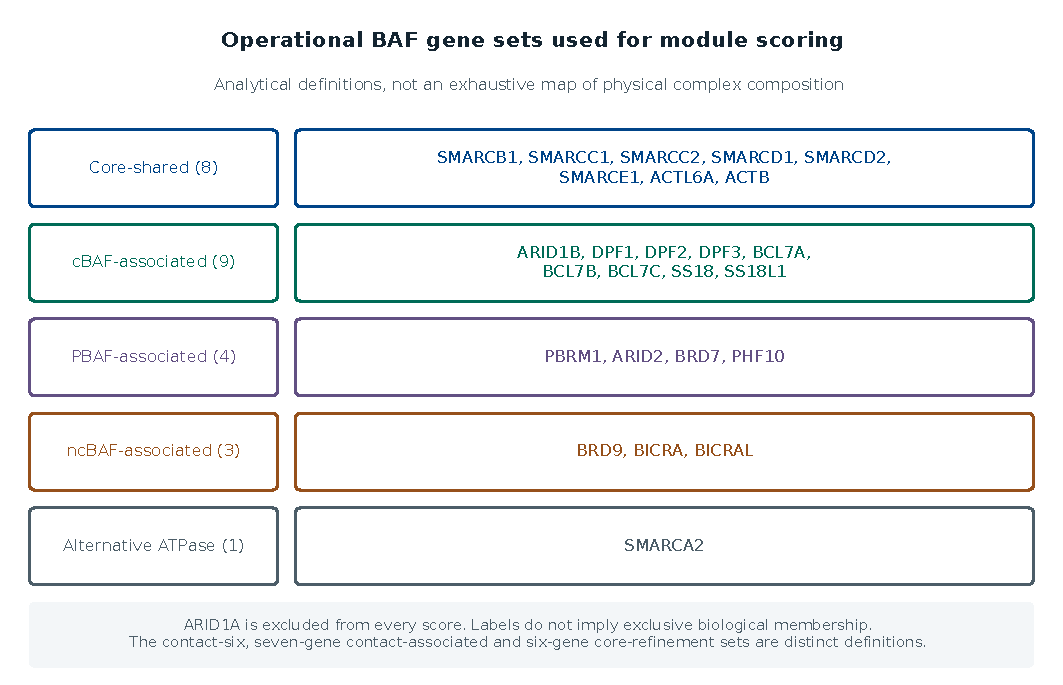
\includegraphics[width=\textwidth,height=0.720\textheight,keepaspectratio]{SupplementaryFigureS1.pdf}
\caption*{\textbf{Operational BAF module definitions.} Fixed gene lists used in module scoring are shown with their gene counts. ARID1A is excluded from every score to avoid anchor self-correlation. The terms core-shared, cBAF-associated, PBAF-associated and ncBAF-associated identify analytical sets; they do not assert exhaustive or exclusive physical membership. In particular, the cBAF-associated label must not be interpreted as cBAF-only localization. The six experimentally resolved contacts, the seven-gene contact-associated set that additionally includes integrative-model-supported SMARCC1, and the six-gene refined core are distinct sets described separately in the text.}
\end{figure}

\clearpage
\section*{Supplementary Figure S2}
\begin{figure}[H]
\centering
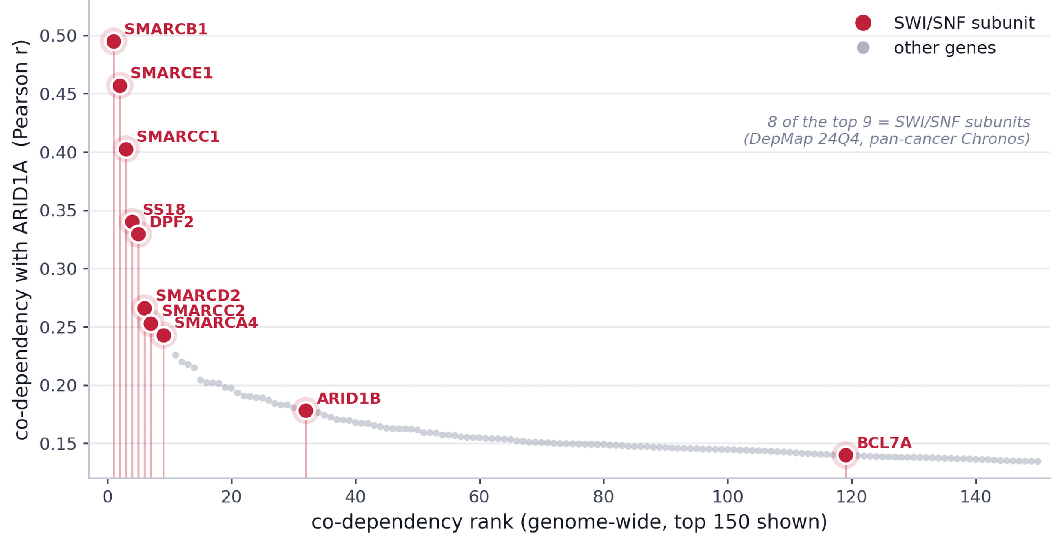
\includegraphics[width=\textwidth,height=0.720\textheight,keepaspectratio]{SupplementaryFigureS2.pdf}
\caption*{\textbf{Genome-wide ARID1A co-dependency landscape in DepMap 24Q4.} The top 150 genes ranked by pan-cancer Pearson co-dependency with ARID1A are shown. SWI/SNF genes are highlighted; eight of the top nine genes belong to this family. Pearson correlations in this ranking are distinct from the Spearman module analyses. Continuous co-dependency does not test ARID1A-loss-conditioned synthetic lethality.}
\end{figure}

\clearpage
\section*{Supplementary Figure S3}
\begin{figure}[H]
\centering
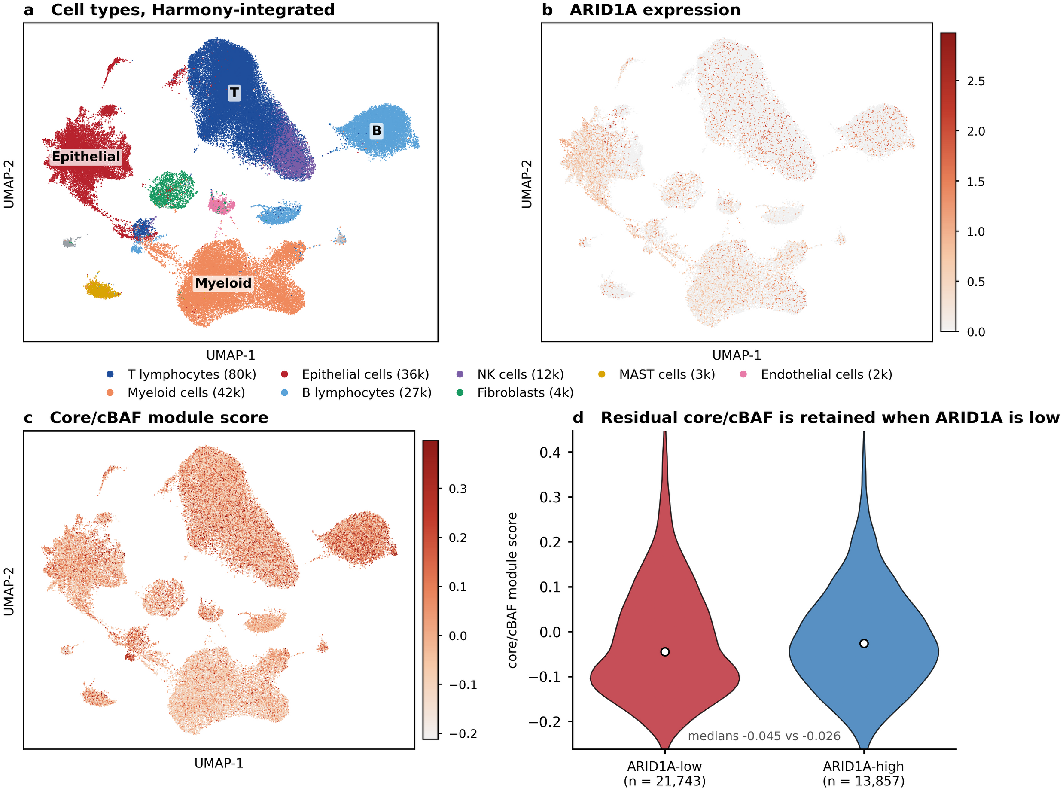
\includegraphics[width=\textwidth,height=0.720\textheight,keepaspectratio]{SupplementaryFigureS3.pdf}
\caption*{\textbf{Single-cell expression context in GSE131907.} Panels show (a) annotated cell types in the Harmony-integrated representation; (b) ARID1A RNA expression; (c) core/cBAF expression-module score; and (d) a descriptive ARID1A-low versus ARID1A-high cell-level split with the original cell counts and medians. These expression measurements are not genetic perturbations. The cell-level split is descriptive and must not be treated as independent patient replication or evidence of cBAF assembly. Annotation-sensitive patient-level estimates are reported separately in the patient-aggregation robustness figure.}
\end{figure}

\clearpage
\section*{Supplementary Figure S4}
\begin{figure}[H]
\centering
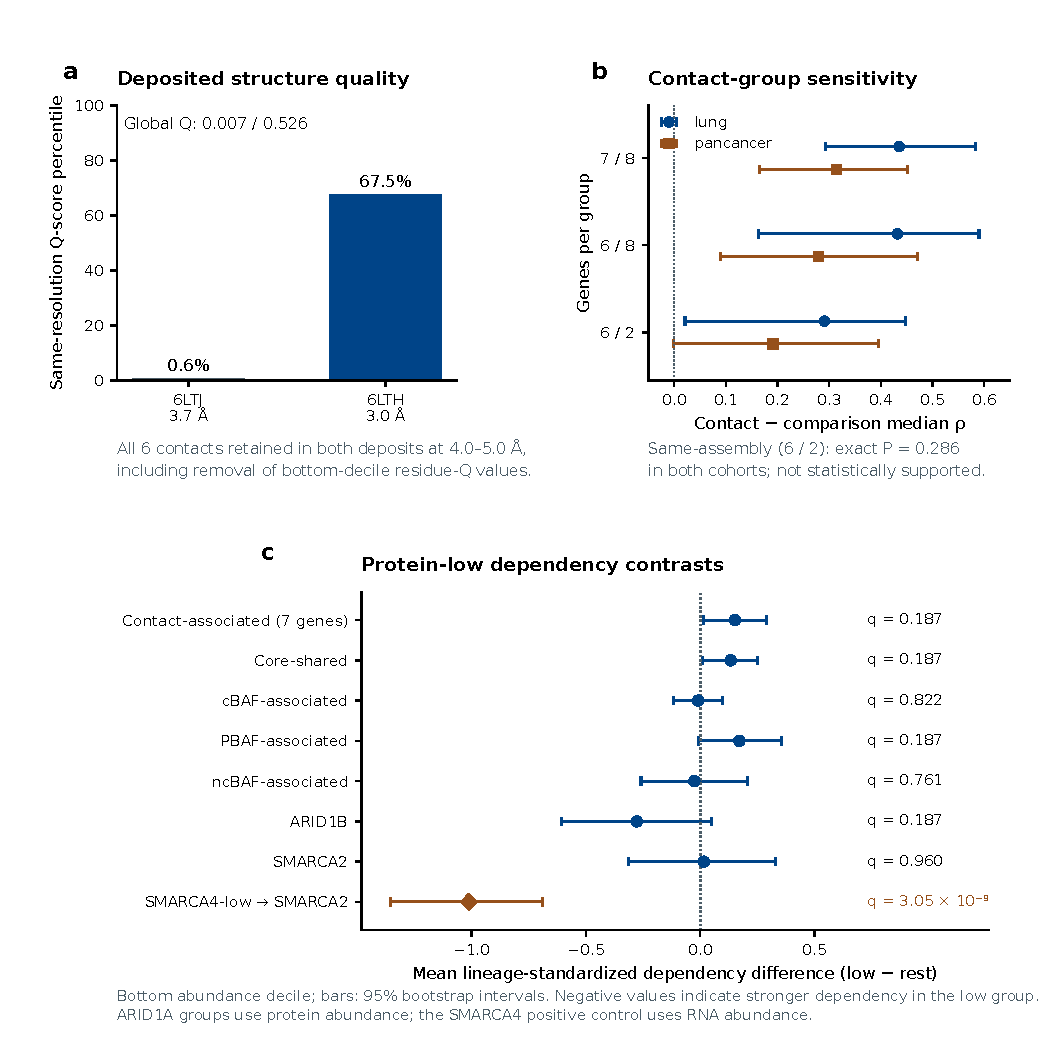
\includegraphics[width=\textwidth,height=0.584\textheight,keepaspectratio]{SupplementaryFigureS4.pdf}
\caption*{\textbf{Structural quality and abundance-defined dependency sensitivity.} (a) Global map--model Q-score same-resolution percentiles for the deposited 6LTJ and 6LTH structures. All six experimentally resolved ARID1A contact calls persisted in both structures at 4.0, 4.5 and 5.0\,\AA{} and after excluding bottom-decile residue-Q values. This robustness does not erase the poor global quality of 6LTJ. (b) median co-dependency differences for the seven-gene contact-associated versus eight-gene comparison partition, the six experimentally resolved contacts versus eight comparisons, and the six-versus-two partition restricted to subunits physically present in 6LTJ. Points show lung and pan-cancer estimates; bars show the 95\% bootstrap intervals. The small six-versus-two comparison remains unsupported by exact two-sided testing ($P=0.286$ in each cohort); bootstrap intervals and exact tests summarize different procedures. (c) Dependency contrasts for the lowest ARID1A protein decile versus remaining measured models, with all seven tested modules or individual comparators retained. The seven-gene contact-associated set additionally includes integrative-model-supported SMARCC1. No ARID1A-protein-low comparison survives within-threshold BH correction. The SMARCA4-low--SMARCA2 positive control uses SMARCA4 RNA abundance and correction across abundance thresholds, and is not protein-defined. Points are mean differences in within-lineage standardized dependency; bars are 95\% percentile-bootstrap intervals (20,000 resamples). Negative differences indicate stronger dependency in the low group.}
\end{figure}

\clearpage
\section*{Supplementary Figure S5}
\begin{figure}[H]
\centering
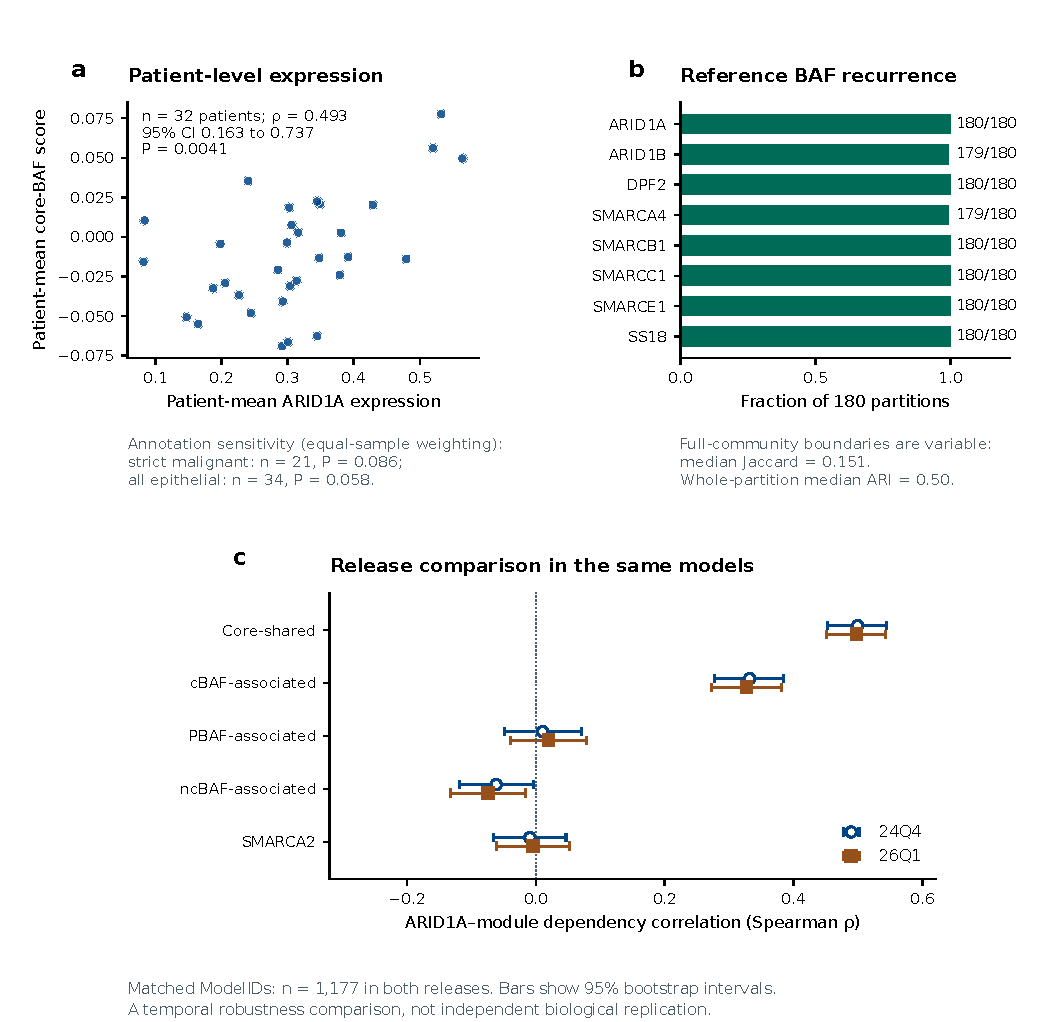
\includegraphics[width=\textwidth,height=0.646\textheight,keepaspectratio]{SupplementaryFigureS5.pdf}
\caption*{\textbf{Patient aggregation, network stability and release-matched robustness.} (a) ARID1A expression versus the core-BAF score after equal-sample patient aggregation of 30,377 annotated tumour-associated epithelial cells from GSE131907. Each point is one patient ($n=32$); the Spearman estimate and patient-bootstrap 95\% interval are displayed. The strict-malignant and all-epithelial, equal-sample sensitivity analyses are reported alongside the primary annotation and remain unsupported at $P<0.05$. (b) Recurrence of the eight BAF genes in the reference ARID1A community across 180 parameter-and-seed partitions. These are the reference-community BAF genes, not all BAF genes. Their recurrence is high, while the full community boundary is variable (median Jaccard 0.151); partition ARI is a separate whole-network summary. (c) Fixed operational-module correlations in DepMap 24Q4 and 26Q1 using the same 1,177 ModelIDs. Points show Spearman correlations and bars their 95\% bootstrap intervals; small vertical offsets separate releases, while connecting segments pair their central estimates. Shared models make this a temporal robustness comparison, not independent biological replication.}
\end{figure}

\clearpage
\section*{Supplementary Figure S6}
\begin{figure}[H]
\centering
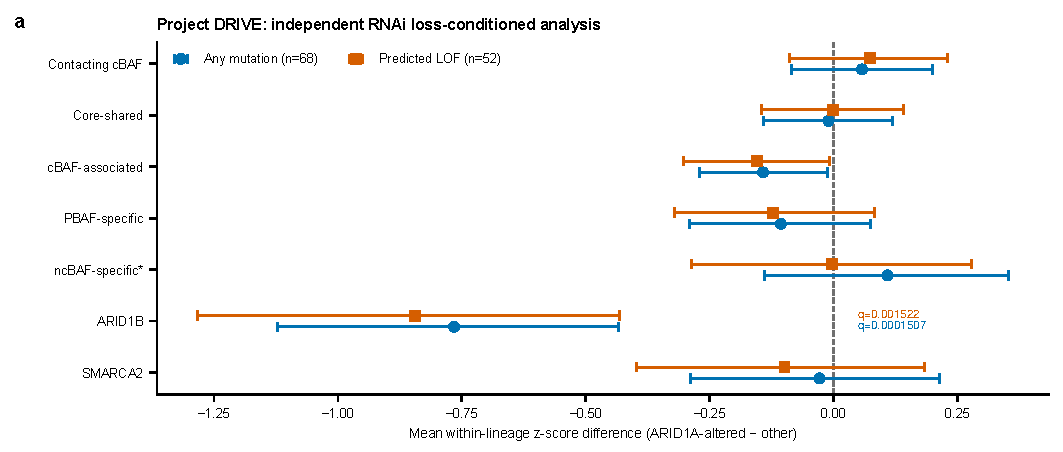
\includegraphics[width=\textwidth,height=0.676\textheight,keepaspectratio]{SupplementaryFigureS6.pdf}
\caption*{\textbf{Project DRIVE RNAi loss-conditioned dependency analysis.} Deep-RNAi viability scores were standardized within 17 lineages represented by at least eight models (354 usable models). Points show mean within-lineage dependency-$z$ differences between ARID1A-altered and other models; bars are 95\% percentile-bootstrap intervals from 20,000 resamples (seed 20260902). Negative values indicate stronger dependency in altered models. ARID1B survives BH correction for both any annotated mutation (68 altered models; $\Delta z=-0.765$, $q=1.51\times10^{-4}$) and predicted loss of function (52 models; $\Delta z=-0.844$, $q=0.00152$). The cBAF-associated module remains unsupported after correction ($q=0.093$ and 0.139). Module coverage is incomplete: six of nine cBAF-associated genes and one of three ncBAF-associated genes were measured; the asterisk marks limited ncBAF coverage. Module labels are operational rather than claims of exclusive physical membership. Published sustained-fitness screens are presented separately with their full current analyses.}
\end{figure}

\clearpage
\section*{Supplementary Figure S7}
\begin{figure}[H]
\centering
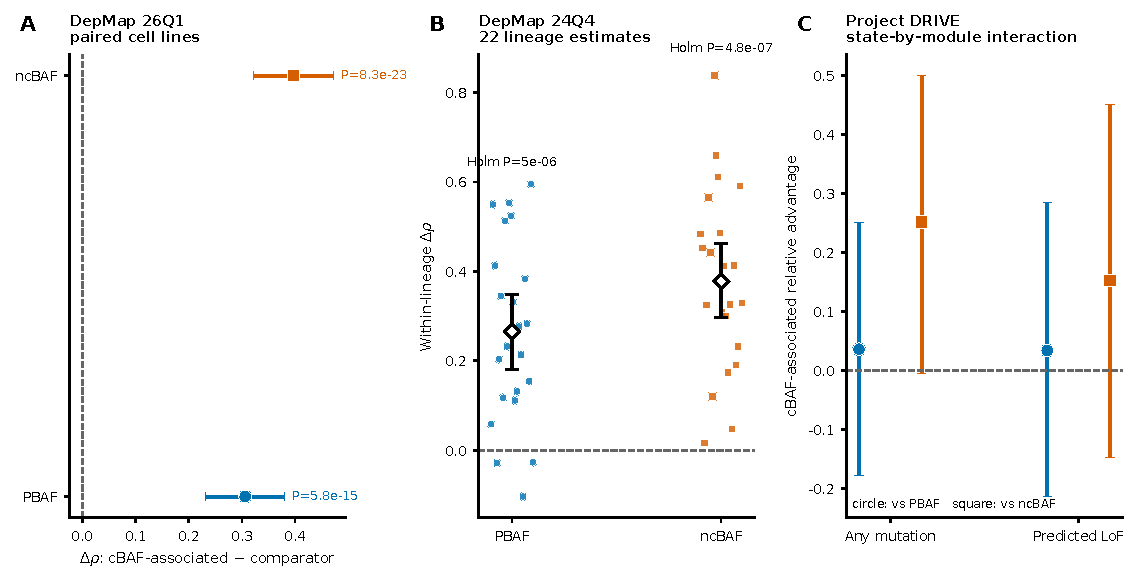
\includegraphics[width=\textwidth,height=0.639\textheight,keepaspectratio]{SupplementaryFigureS7.pdf}
\caption*{\textbf{Direct comparisons distinguish the cBAF-associated gene
score from prespecified comparator modules.} (\textbf{A}) On the same 1{,}208
DepMap 26Q1 models, points are the paired difference between ARID1A--cBAF and
ARID1A--comparator Spearman correlations; bars are 95\% model-bootstrap
intervals. Labels are Holm-adjusted one-sided $P$ values from rank-normalised
within-model module contrasts. (\textbf{B}) Raw within-lineage differences from
22 DepMap 24Q4 lineages (at least 15 models each). Small points are lineages; diamonds and bars are the
lineage mean and 95\% lineage-bootstrap interval. Exact mean sign-flip tests are
Holm-adjusted across PBAF and ncBAF comparisons. (\textbf{C}) Project DRIVE
ARID1A-state-by-module difference-in-differences, plotted so positive values
support stronger cBAF-relative dependency. Circles compare cBAF with PBAF and
squares with ncBAF; bars are 95\% cell-line bootstrap intervals. Only the
any-mutation cBAF-versus-ncBAF comparison passes lineage-stratified permutation
correction (Holm $P=0.0482$); the other three are corrected-null. Panels test
association differences between operational gene groupings, not exclusive cBAF
assembly membership or long-term causal dependence. All resampling used
20{,}000 iterations and seed 20260902.}
\end{figure}

\clearpage
\section*{Supplementary Figure S8}
\begin{figure}[H]
\centering
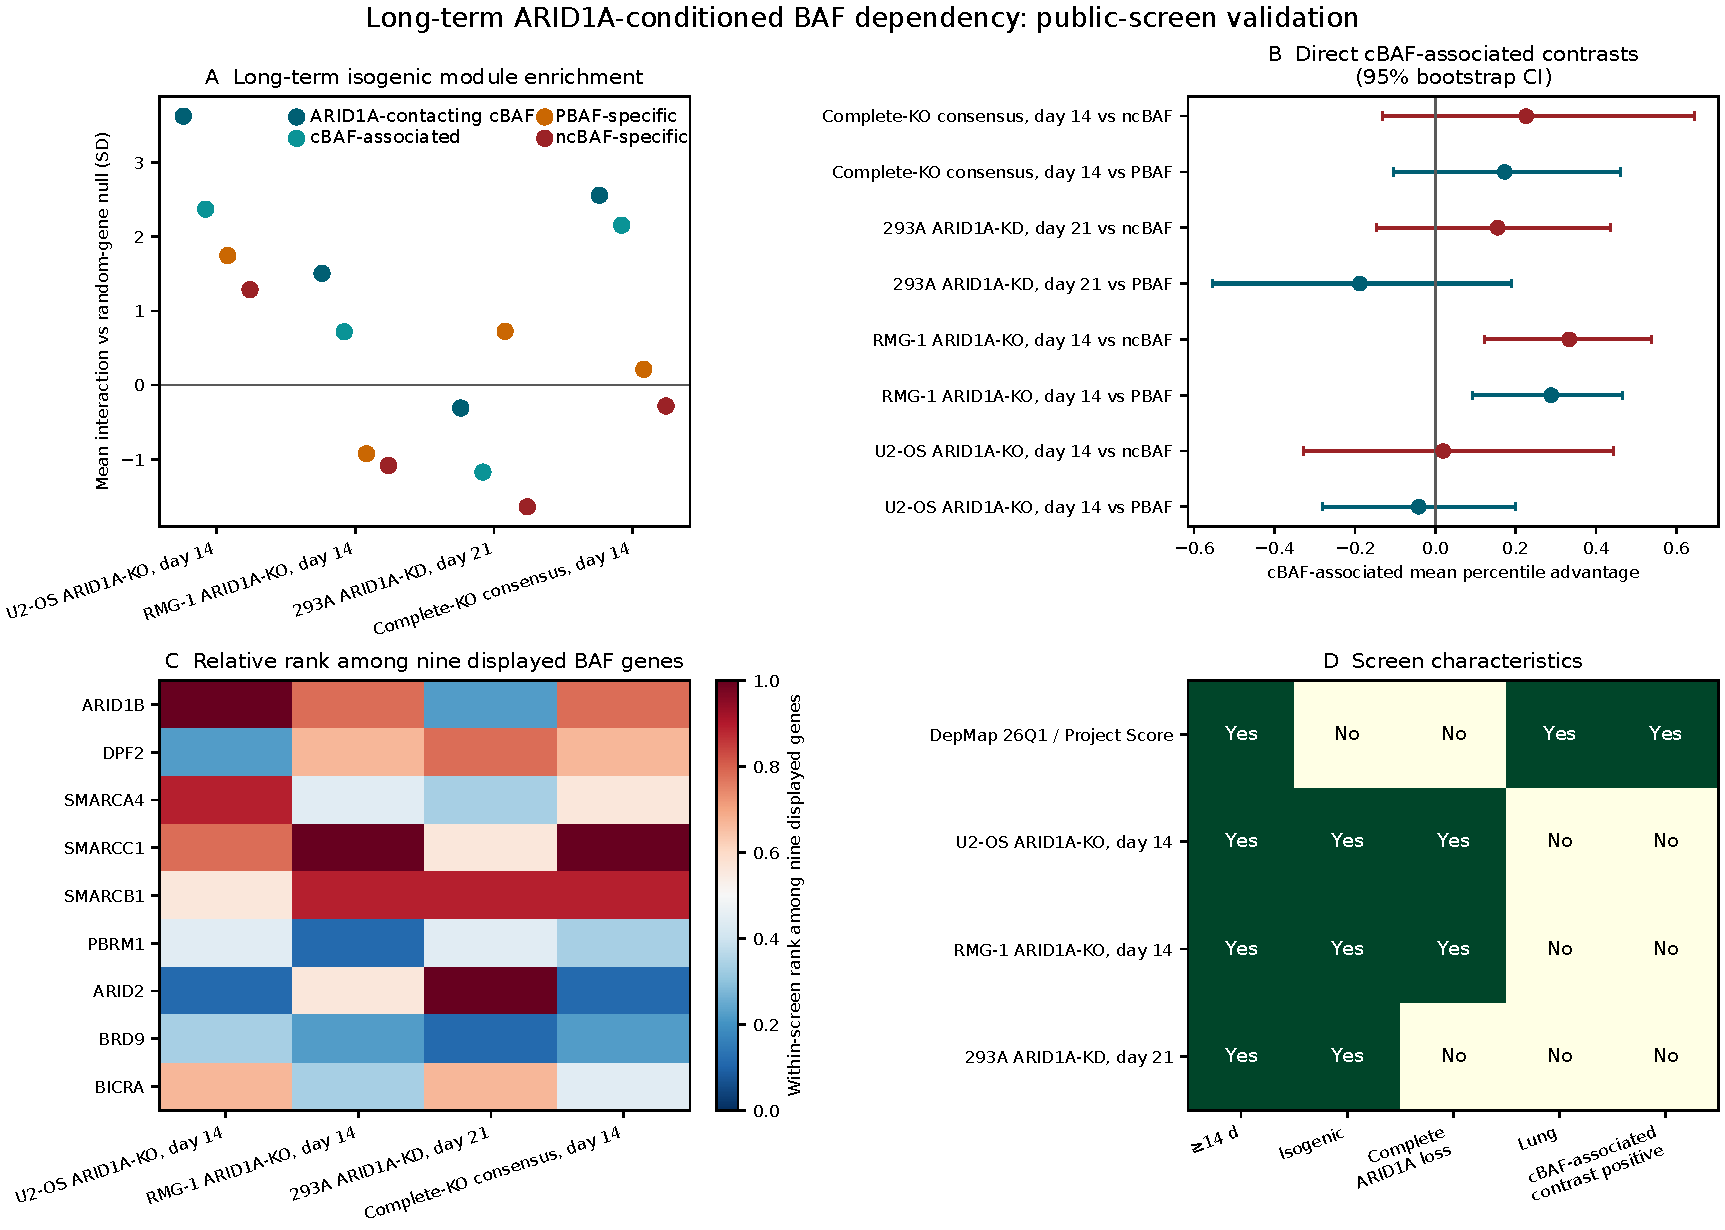
\includegraphics[width=\textwidth,height=0.606\textheight,keepaspectratio]{SupplementaryFigureS8.pdf}
\caption*{\textbf{Published sustained-fitness screens distinguish gene-set enrichment
from direct sub-complex comparisons.}
(\textbf{A}) Module mean interaction relative to 100{,}000 whole-genome,
size-matched random gene sets; positive standardised values indicate stronger
dependency in the ARID1A-deficient condition. U2-OS and RMG-1 were complete
ARID1A-knockout screens with 14-day endpoints; 293A was a 21-day ARID1A-KD
screen with a reported residual protein species. The complete-KO consensus
averages within-screen gene percentiles across U2-OS and RMG-1. (\textbf{B})
Direct cBAF-associated-versus-PBAF/ncBAF mean percentile differences and 95\%
gene-bootstrap intervals; positive values favour cBAF, but none survived Holm
correction. (\textbf{C}) Relative interaction ranks among the nine displayed
BAF genes within each screen, not genome-wide percentiles. This illustrative
heatmap is separate from the genome-wide reference in panel a.
(\textbf{D}) Screen characteristics separating assay duration, isogenicity,
complete ARID1A loss, lung origin and a multiplicity-corrected direct cBAF
contrast. The complete-KO consensus was significant relative to random genes for
ARID1A-contacting cBAF (BH $q=0.0204$) and cBAF-associated genes ($q=0.0287$),
whereas PBAF and ncBAF were null; direct cBAF competition remained
corrected-null (minimum Holm $P=0.327$). Seed 20260902.}
\end{figure}

\clearpage
\section*{Supplementary Figure S9}
\begin{figure}[H]
\centering
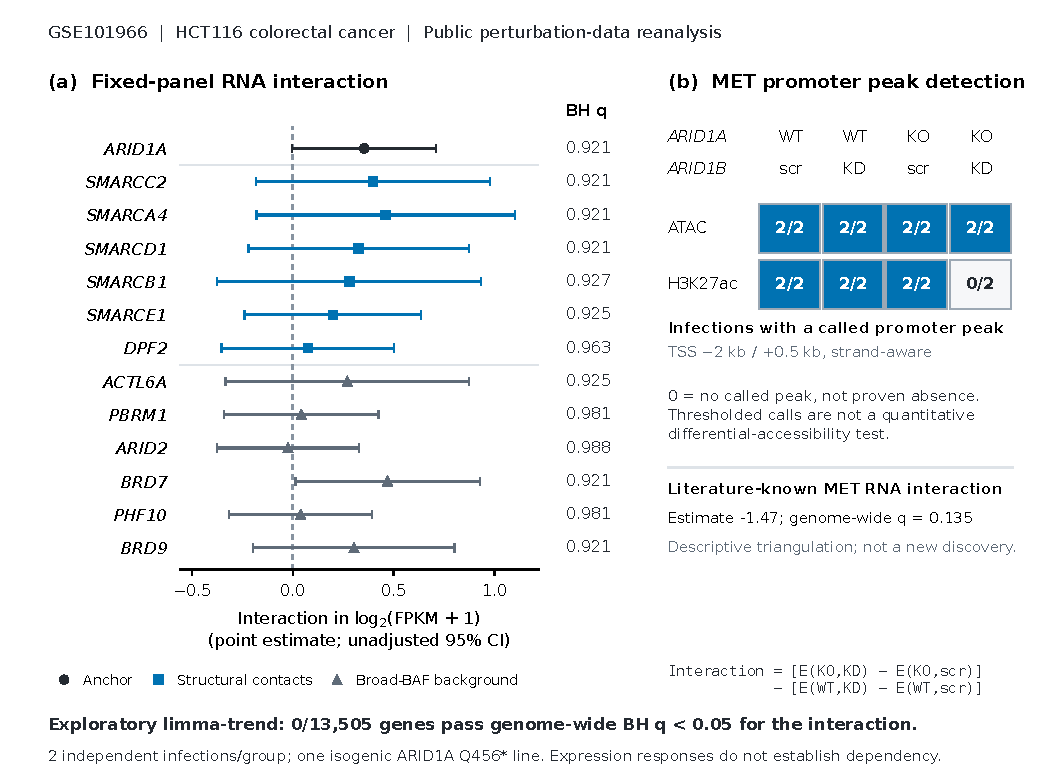
\includegraphics[width=\textwidth,height=0.550\textheight,keepaspectratio]{SupplementaryFigureS9.pdf}
\caption*{\textbf{Exploratory molecular-response analysis of public
ARID1A/ARID1B perturbations.} (\textbf{a}) The fixed ARID1A anchor, six
experimental structural-contact subunits and six broad-BAF background subunits
are shown without selection by their effects. Points and bars are
genotype-by-ARID1B-knockdown coefficients and unadjusted 95\% moderated-model
intervals from limma-trend on log$_2$(FPKM+1). The interaction is
$[E(\mathrm{KO},\mathrm{KD})-E(\mathrm{KO},\mathrm{scr})]-
[E(\mathrm{WT},\mathrm{KD})-E(\mathrm{WT},\mathrm{scr})]$, where $E$ is
transformed expression. BH correction covered all 13{,}505 tested genes;
none passed $q<0.05$. The intervals are not simultaneous or FDR-controlled.
(\textbf{b}) Number of the two infections with a separately called ATAC or
H3K27ac peak overlapping the MET promoter (strand-aware TSS $-2$\,kb to
$+0.5$\,kb). Zero means non-detection under the original calling threshold,
not proven absence of accessibility or acetylation. These peak lists do not
provide a quantitative differential-chromatin test. MET was a literature-known
candidate in the source study, included as secondary descriptive evidence, not
a new discovery. GSE101966 (Kelso et al., eLife 2017,
doi:10.7554/eLife.30506) used HCT116 colorectal cancer cells, two independent
lentiviral infections per condition and one isogenic ARID1A Q456* line;
infections are not independent knockout clones. This FPKM-based re-analysis is
exploratory and does not establish lung-cancer generalizability or cellular
dependency. WT, wild type; KO, knockout; KD, knockdown; scr, scrambled shRNA;
TSS, transcription start site.}
\end{figure}

\clearpage
\section*{Supplementary Figure S10}
\begin{figure}[H]
\centering
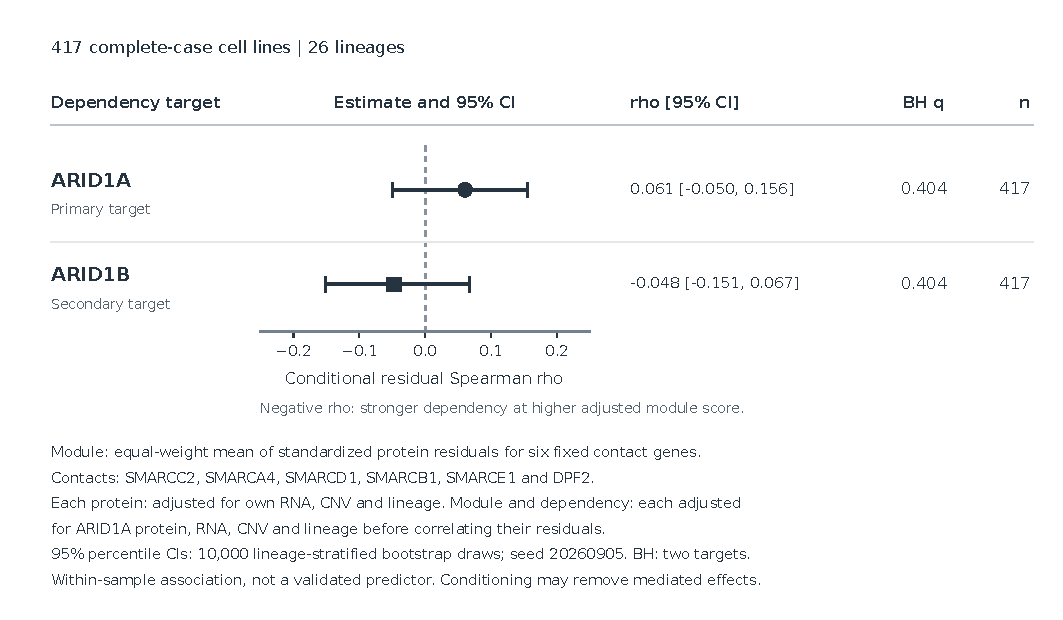
\includegraphics[width=\textwidth,height=0.629\textheight,keepaspectratio]{SupplementaryFigureS10.pdf}
\caption*{\textbf{Conditional associations between the six-contact protein
module and ARID1A/ARID1B dependency.} The same 417 complete-case cell lines
from 26 lineages are used for both targets. Each of the six contacting
proteins was first residualized on its own RNA, CNV and lineage, standardized
on the common complete-case panel, and combined with equal weights. The
module score and each CRISPR dependency outcome were then residualized on
ARID1A protein, RNA, CNV and lineage before calculating Spearman correlation.
Points are conditional correlations; bars are 95\% percentile intervals from
10{,}000 lineage-stratified, shared-row bootstrap draws that refit every model
(seed 20260905). Two-sided centred-bootstrap approximate $P$ values were
BH-corrected across the two targets. Both intervals cross zero and both
$q=0.404$; neither target shows a corrected association. Negative correlation
would mean stronger dependency at a higher module score. This is an
observational complete-case analysis, not an externally validated predictor.
Conditioning on the anchor may remove mediated associations, and complete-case
selection may affect generalizability; non-significance does not prove the
absence of all biological relationships.}
\end{figure}

\clearpage
\section*{Supplementary Figure S11}
\begin{figure}[H]
\centering
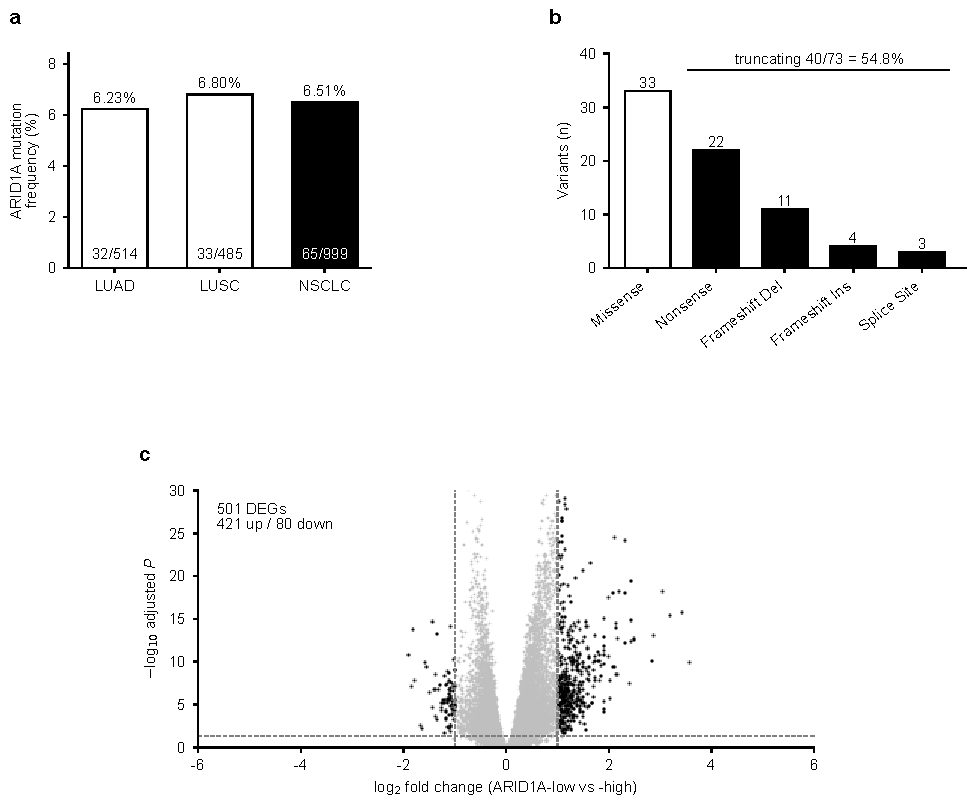
\includegraphics[width=\textwidth,height=0.720\textheight,keepaspectratio]{SupplementaryFigureS11.pdf}
\caption*{\textbf{ARID1A is recurrently mutated and frequently truncated in NSCLC.}
(\textbf{a}) Mutation frequency in TCGA-LUAD, TCGA-LUSC and the combined NSCLC
cohort; counts give mutated cases over cohort size. (\textbf{b}) Variant
classification spectrum; filled bars are truncating classes. (\textbf{c}) Volcano
plot of ARID1A-low versus ARID1A-high tertile differential expression; filled
points pass adjusted $P < 0.05$ and $|\log_2\mathrm{FC}| > 1$.}
\end{figure}

\clearpage
\section*{Supplementary Figure S12}
\begin{figure}[H]
\centering
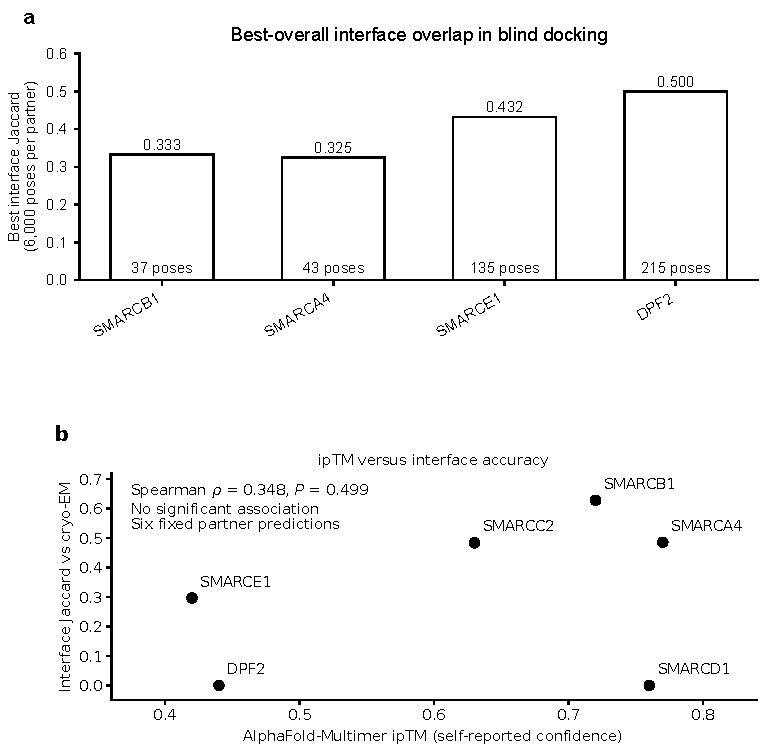
\includegraphics[width=\textwidth,height=0.720\textheight,keepaspectratio]{SupplementaryFigureS12.pdf}
\caption*{\textbf{Computational structural cross-validation.} (\textbf{a}) Blind
docking interface recovery; the best Jaccard over all 6{,}000 poses per partner,
with the number of near-native poses ($J \ge 0.2$) annotated. (\textbf{b})
AlphaFold-Multimer interface reproduction against self-reported ipTM for the six
contacting partners, using the fixed rank-1 predictions and sequence-resolved residue crosswalks for discontinuous ARID1A inputs. The six-point Spearman
association is $\rho=0.348$, $P=0.499$; input coverage differs between partners.}
\end{figure}

\clearpage
\section*{Supplementary Table S1}
Complex-module co-dependency with ARID1A. The anchor is excluded from
every module (Methods in the main article).

{\small
\begin{tabular}{lccccc}
\toprule
\textbf{Module} & \textbf{Subunits} & \textbf{Lung $\rho$} & \textbf{$P$}
 & \textbf{Pan-cancer $\rho$} & \textbf{$P$} \\
\midrule
Core-shared    & 8 & $+0.447$ & $1.2\times10^{-7}$ & $+0.461$ & $3.1\times10^{-50}$ \\
cBAF-associated  & 9 & $+0.456$ & $6.2\times10^{-8}$ & $+0.307$ & $1.0\times10^{-21}$ \\
PBAF-specific  & 4 & $-0.123$ & $0.166$            & $-0.012$ & $0.720$ \\
ncBAF-specific & 3 & $-0.157$ & $0.076$            & $-0.110$ & $8.1\times10^{-4}$ \\
Alt.\ ATPase (SMARCA2) & 1 & $-0.122$ & $0.170$    & $-0.002$ & $0.958$ \\
\bottomrule
\end{tabular}
}
\clearpage
\section*{Supplementary methods and validation results}
\label{sec:supp_r15}

Prediction, matched-control and HAP1 analyses use separately defined
observational units, endpoints and correction families. The analysis
specifications were fixed before fitting or testing, but were not
prospectively registered. Complete predictions, fixed-panel results,
sample-attrition records and source manifests accompany Supplementary Data~S1.

\paragraph{Grouped prediction.}
The target was observed in all 1{,}178 models. There were 1{,}129 PatientID
groups, including 41 patients with multiple models, and no missing patient
or lineage annotations. No patient crossed lineages, leaving 30 connected
patient--lineage groups. Each model was held out once under each scheme.
The selected single gene was SMARCB1 in all ten folds. Both schemes ranked
SMARCB1, SMARCE1, SMARCC1, DPF2 and ARID1B as the five largest mean absolute
OOF SHAP features. Features not selected in a fold contribute zero to its
aggregate importance. Correlated genes can share attribution, and this
ranking is not evidence of cBAF-exclusive function or causality.

\renewcommand{\thetable}{S\arabic{table}}
\setcounter{table}{1}
\begin{table}[htbp]
\centering
\small
\caption{\textbf{Fixed-model prediction with patient- and lineage-group holdout.}}
\label{tab:sr_r15_ml}
\resizebox{\textwidth}{!}{%
\begin{tabular}{llrrrr}
\toprule
Scheme & Model & Pooled OOF $R^2$ & Fold $R^2$, mean $\pm$ SD & OOF RMSE & OOF MAE \\
\midrule
Patient & XGBoost & 0.3841 & $0.3796\pm0.0428$ & 0.2210 & 0.1696 \\
Patient & Ridge ($\alpha=10$) & 0.1461 & $0.1342\pm0.0859$ & 0.2602 & 0.2009 \\
Patient & Training-selected single-gene OLS & 0.2408 & $0.2368\pm0.0256$ & 0.2453 & 0.1872 \\
Patient & Training mean & $-0.0016$ & $-0.0043\pm0.0051$ & 0.2818 & 0.2157 \\
\midrule
Lineage component & XGBoost & 0.3620 & $0.3597\pm0.0380$ & 0.2249 & 0.1735 \\
Lineage component & Ridge ($\alpha=10$) & 0.0740 & $0.0477\pm0.0609$ & 0.2709 & 0.2101 \\
Lineage component & Training-selected single-gene OLS & 0.2353 & $0.2260\pm0.0489$ & 0.2462 & 0.1880 \\
Lineage component & Training mean & $-0.0071$ & $-0.0119\pm0.0118$ & 0.2825 & 0.2159 \\
\bottomrule
\end{tabular}}
\par\smallskip
\begin{minipage}{\textwidth}
\footnotesize
All rows use 1{,}178 OOF observations and five test folds. Fold SD is descriptive
variation across the five folds, not a confidence interval. The test-fold
outcome mean defines each fold's $R^2$ denominator, whereas the pooled
denominator uses the overall outcome mean. These two estimands are not
interchangeable. RMSE and MAE have gene-effect units. No model was tuned or
selected on these results; numerical differences are descriptive, without
a model-superiority test. Both schemes reuse the same DepMap public resource,
not an independent external cohort. Source:
\texttt{ml/run\_v1/performance\_summary.csv} in Supplementary Data~S1.
\end{minipage}
\end{table}

\paragraph{Matched controls and sample attrition.}
All 27{,}700 attempted comparisons were retained in the analysis inventory;
25{,}762 were evaluable. There were 925 strong-null
matching failures and 1{,}013 size-null failures from insufficient paired
complete cases. The strict primary set requires all ten splits and five
replicates of both null types to be evaluable, retaining 112 complexes in
51 of the 108 pre-frozen overlap families. Retained complexes had median
size seven, versus ten among exclusions. Available-case summaries remain
descriptive and cannot replace the primary complete set.

The final primary training populations comprised 5{,}600 real--strong and
5{,}600 real--size pairs. For the module means of the three non-missingness
matching variables (dependency mean, SD and strong-dependency fraction),
average absolute standardized differences were 0.0281, 0.0352 and 0.0239
for strong controls, versus 1.2317, 1.2257 and 1.1505 for size controls.
Of 42{,}400 primary strong-match gene pairs, one final-training SD difference
exceeded the original 0.5 caliper (maximum 0.5225). Original matching did
satisfy the caliper; this later deviation arose after complete-case restriction.
Both arms have zero missingness after that restriction by construction.
These checks support better marginal balance, not matching of network degree,
covariance, lineage structure or biological membership.

\begin{table}[htbp]
\centering
\small
\caption{\textbf{All eight prespecified tests in the strong-null analysis.}}
\label{tab:sr_r15_null}
\resizebox{\textwidth}{!}{%
\begin{tabular}{lllrrrr}
\toprule
Unit & Null & Endpoint & Mean difference & Nominal 95\% interval & Two-sided $P$ & BH $q$ \\
\midrule
Family ($n=51$) & Strong & Identity & 0.10948 & $[0.02768,0.19108]$ & 0.01135 & 0.01513 \\
Family ($n=51$) & Strong & Gain & $-0.00242$ & $[-0.00812,0.00365]$ & 0.42718 & 0.42718 \\
Family ($n=51$) & Size & Identity & 0.18322 & $[0.10469,0.25781]$ & 0.00010 & 0.00020 \\
Family ($n=51$) & Size & Gain & 0.00401 & $[-0.00135,0.00973]$ & 0.16944 & 0.19365 \\
\midrule
Complex ($n=112$) & Strong & Identity & 0.20536 & $[0.14536,0.26375]$ & 0.00005 & 0.00013 \\
Complex ($n=112$) & Strong & Gain & 0.00754 & $[0.00250,0.01283]$ & 0.00590 & 0.00944 \\
Complex ($n=112$) & Size & Identity & 0.26071 & $[0.20321,0.31821]$ & 0.00005 & 0.00013 \\
Complex ($n=112$) & Size & Gain & 0.01259 & $[0.00765,0.01770]$ & 0.00005 & 0.00013 \\
\bottomrule
\end{tabular}}
\par\smallskip
\begin{minipage}{\textwidth}
\footnotesize
Differences are real minus matched null. Identity denotes concordance of
the training-selected removal with the test-half best removal for the fixed
training-selected anchor. Gain denotes held-out correlation gain from that
training-selected removal. Primary inference weights the 51 overlap families
equally; direct complex-level inference is a sensitivity analysis and cannot
replace the family-level null result for gain. Intervals use 10{,}000 bootstrap
draws; $P$ values use 20{,}000 two-sided sign-flip draws with a $+1$ correction,
and are not zero even where rounded to 0.00005. BH correction covers all
eight rows together; intervals are not multiplicity-adjusted. Source:
\texttt{strong\_null/r15\_primary\_inference.csv} in Supplementary Data~S1.
\end{minipage}
\end{table}

\paragraph{HAP1 fixed-panel genetic interactions.}
The published GIN019 screen used HAP1 Clone~33 with three technical endpoints.
All 17{,}804 source gene scores and the complete fixed panels were retained;
the three direct contrasts are reported below. The five secondary competitive
negative-hit enrichment tests were corrected together by BH.

\begin{table}[htbp]
\centering
\small
\caption{\textbf{Complete fixed-panel HAP1 genetic-interaction contrasts.}}
\label{tab:sr_r15_hap1}
\resizebox{\textwidth}{!}{%
\begin{tabular}{lrrrrr}
\toprule
Comparison & Genes, A/B & $\Delta$ mean $(-\mathrm{qGI})$ & Allocations & Exact two-sided $P$ & Holm $P$ \\
\midrule
Contact / broad BAF background & 6/6 & 0.09017 & 924 & 0.53680 & 0.58636 \\
cBAF-associated / PBAF & 9/4 & 0.37731 & 715 & 0.25734 & 0.58636 \\
cBAF-associated / ncBAF & 9/3 & 0.55622 & 220 & 0.19545 & 0.58636 \\
\bottomrule
\end{tabular}}
\par\smallskip
\begin{minipage}{\textwidth}
\footnotesize
A positive contrast denotes stronger ARID1A-loss-conditioned depletion
in panel A. Gene-label allocations were exhaustively enumerated and
absolute-effect extremeness defined the two-sided test; Holm adjustment
covers these three comparisons together. All panels were complete. The
exchangeable units are genes under a competitive null, not independent
knockout clones. The data represent one HAP1 clone with three technical
endpoints. The broad BAF background is not a set of verified physical
non-contacts in the same assembly. Source:
\texttt{hap1/primary\_direct\_contrasts.csv} in Supplementary Data~S1.
\end{minipage}
\end{table}

The negative-hit background comprised 17{,}803 finite scored non-anchor genes
and 249 author-defined hits ($\mathrm{qGI}<-0.3$, author FDR$<0.1$).
ARID1B was the sole hit among the nine cBAF-associated genes
(Fisher $P=0.11909$, five-set BH $q=0.59543$).
Its source qGI was $-1.724$ with author FDR
$4.851092\times10^{-12}$, and its alternative-guide ARID1A-minus-WT dLFC
was $-0.741115$. These values describe a known single-gene interaction in
this model, not a novel pair or a positive whole-module validation.
The complete source FDR columns were retained; the unavailable underlying
gene-level $P$ values were not reverse-engineered or re-corrected in a BAF
subset.

\begingroup\small
S6 is a targeted guide-rescreen library selected using initial hits from five
queries. Although the source article describes 1{,}215 selected genes, both
downloaded S6 tables contain 1{,}214 unique genes; this discrepancy was
recorded without inferring its cause. It covers contact 3/6, broad BAF
background 1/6, cBAF-associated 2/9, PBAF 0/4 and ncBAF 1/3, representing five
of the 22 unique fixed members. Missing members were retained as missing,
not replaced or scored zero, and available-case directions were not treated
as full independent module validation. No gene-level rescreen FDR was
available.
\endgroup

\clearpage
\section*{Supplementary Figure S13}
\begin{figure}[H]
\centering
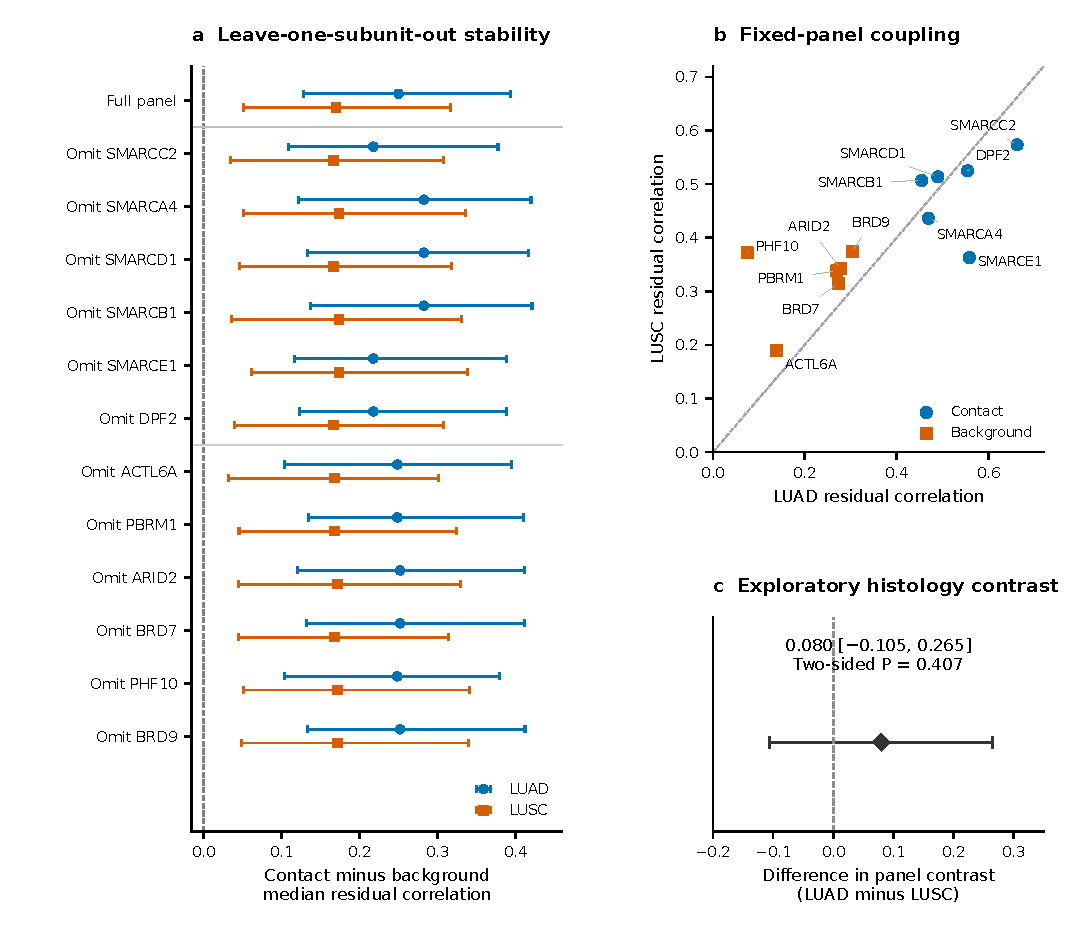
\includegraphics[width=\textwidth,height=0.66\textheight,keepaspectratio]{SupplementaryFigureS13.pdf}
\caption*{\textbf{Exploratory cross-histology protein-coupling robustness.} (\textbf{a}) Full-panel and leave-one-subunit-out contact-minus-background median residual-correlation differences in CPTAC LUAD ($n=108$) and LUSC ($n=107$). Points are estimates; bars are nominal 95\% shared-row bootstrap intervals (10,000 archived covariate-refitted draws), not simultaneous intervals. Each subunit is removed only from its assigned panel. (\textbf{b}) All 12 fixed-panel protein correlations after own-RNA, own-copy-number and tumour-purity adjustment; colour and shape distinguish contact and background proteins. Each point is a protein, not a patient. The dashed line is the identity. (\textbf{c}) LUAD-minus-LUSC difference in the panel contrast, with a percentile 95\% interval and two-sided centred-bootstrap $P$. Entire bootstrap-row indices were independently paired between cohorts with a fixed seed. Absence of a significant difference does not demonstrate equivalence. These analyses were added after the primary results were known, introduced no new patients and retained all 12 proteins. Positive coupling also occurs among background proteins; the findings do not establish exclusive cBAF dependence.}
\end{figure}

\clearpage
\section*{Exploratory repeated-support tests in independent tumour cohorts}
The fixed panel contained six experimentally resolved contacts (SMARCC2, SMARCA4, SMARCD1, SMARCB1, SMARCE1 and DPF2) and six broad BAF-family background proteins (ACTL6A, PBRM1, ARID2, BRD7, PHF10 and BRD9). Panel membership was unchanged. Source bootstrap arrays and primary tables were copied from the archived purity-adjusted CPTAC analysis; all six input-file hashes matched the previously submitted Supplementary Data S3. Replay of the full-panel point estimates and intervals agreed within $10^{-12}$. The new computations were run on the authors' remote server; no new biological samples, imputation or synthetic observations were introduced.

For each protein and cohort, a one-sided centred-bootstrap test evaluated positive adjusted protein correlation with ARID1A. The larger of the two cohort-specific $P$ values was the intersection--union repeated-support $P$. Holm correction was applied across all 12 proteins, rather than only the contact panel or nominally positive proteins. The table reports the complete family; the two cohort-specific tail probabilities are retained in Supplementary Data S5. With 10,000 bootstrap draws and a plus-one correction, the minimum cohort-specific probability is $1/10001$; very small values should not be interpreted as precision beyond this Monte Carlo resolution. These approximate bootstrap tests are exploratory and were not pre-specified before inspection of the primary results.

\begin{table}[H]
\centering\small
\caption{\textbf{Exploratory positive protein coupling supported in both tumour cohorts.}}
\label{tab:cross_histology}
\begin{tabular}{llrrrrl}
\toprule
Protein & Panel & LUAD $\rho$ & LUSC $\rho$ & IUT $P$ & Holm $P$ & Both supported \\
\midrule
SMARCC2 & Contact & 0.662 & 0.573 & 0.00010 & 0.00120 & Yes \\
SMARCA4 & Contact & 0.469 & 0.436 & 0.00010 & 0.00120 & Yes \\
SMARCD1 & Contact & 0.489 & 0.514 & 0.00010 & 0.00120 & Yes \\
SMARCB1 & Contact & 0.454 & 0.507 & 0.00010 & 0.00120 & Yes \\
SMARCE1 & Contact & 0.558 & 0.363 & 0.00020 & 0.00140 & Yes \\
DPF2 & Contact & 0.554 & 0.525 & 0.00010 & 0.00120 & Yes \\
ACTL6A & Background & 0.139 & 0.189 & 0.10209 & 0.20418 & No \\
PBRM1 & Background & 0.270 & 0.338 & 0.00080 & 0.00240 & Yes \\
ARID2 & Background & 0.278 & 0.342 & 0.00040 & 0.00200 & Yes \\
BRD7 & Background & 0.273 & 0.315 & 0.00060 & 0.00240 & Yes \\
PHF10 & Background & 0.075 & 0.372 & 0.23528 & 0.23528 & No \\
BRD9 & Background & 0.303 & 0.374 & 0.00020 & 0.00140 & Yes \\
\bottomrule
\end{tabular}
\end{table}

All six contacts and four background proteins met adjusted $P<0.05$ with positive point estimates in both cohorts. This endpoint describes repeated positive coupling, not contact-specific superiority for each gene. All 12 leave-one-subunit-out estimates and nominal intervals are supplied, including omissions from the background panel; the intervals overlap and are not independent validation studies. The single exploratory histology-difference test was evaluated separately, not mixed into the 12-protein Holm family.

Supplementary Data S5 contains the executable analysis, six exact archived input files, all results, the cross-cohort row permutation and verification records. An independent local numerical audit reproduced all 24 cohort-level tail probabilities, all 12 Holm-adjusted probabilities and all 26 full/leave-one-out point estimates. The new analyses do not alter the originally reported primary tests or their multiplicity families.


\clearpage
\section*{Supplementary Figure S14}
\begin{figure}[H]\centering
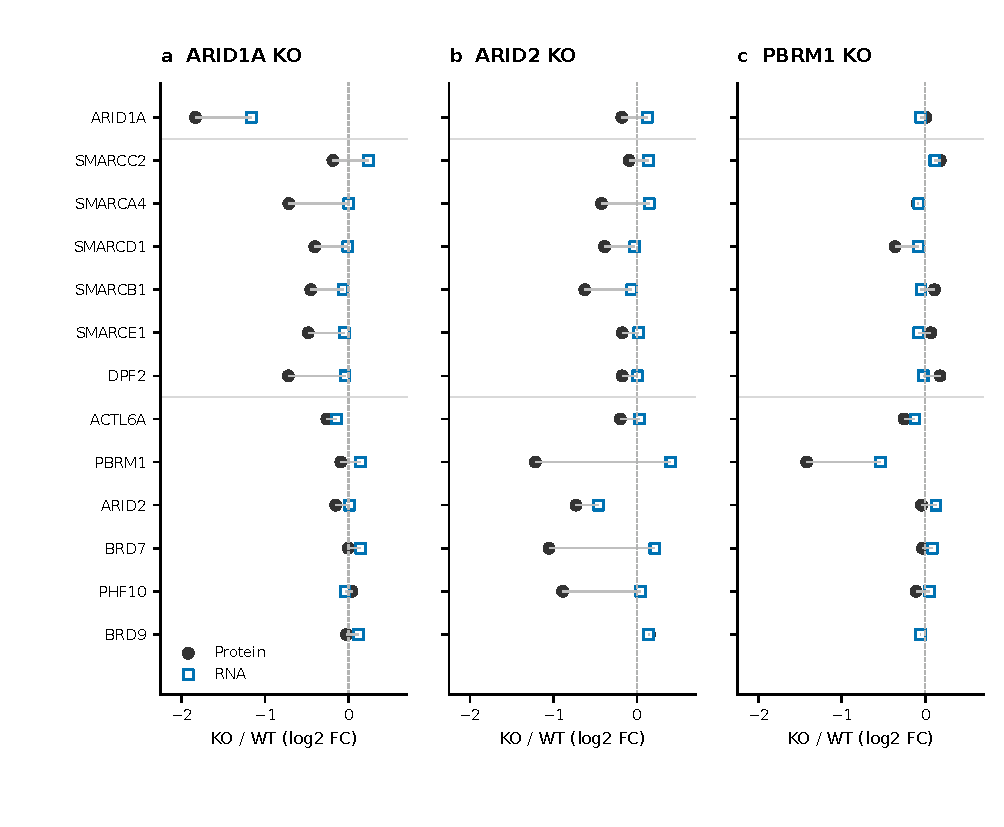
\includegraphics[width=\textwidth,height=0.64\textheight,keepaspectratio]{SupplementaryFigureS14.pdf}
\caption*{\textbf{Complete published iPSC knockout context for the fixed protein panel.} ARID1A (\textbf{a}), ARID2 (\textbf{b}) and PBRM1 (\textbf{c}) knockout versus WT. Filled circles show $\log_2[\mathrm{mean(KO)}/\mathrm{mean(WT)}]$ from the source normalized TMT values (two labelled clones per condition); open squares show the published RNA-seq coefficients. Horizontal segments link two molecular endpoints, not paired replicate observations. All conditions and panel members are retained, with ARID1A displayed separately as the anchor. ARID2 and PBRM1 are themselves members of the fixed background; summaries excluding the perturbed background gene are provided in Supplementary Data S7. Published RNA analysis used six biological replicates per knockout and four WT samples; raw RNA counts were not reanalysed here. Source protein ANOVA tests compare all conditions jointly and are not treated as query-specific probabilities. No new gene- or module-level significance claims are made. The source methods included minimum-intensity handling of missing peptide channels; this cannot be undone from the protein table. Data: Roumeliotis et al., Cell Reports 2017, doi:10.1016/j.celrep.2017.08.010, original Table S6.}
\end{figure}

\clearpage
\section*{Proteome-wide eligibility, ranking and robustness}
The proteome-wide universe required complete protein/RNA/CNV measurement in every purity-complete primary patient. This ensured equal patient counts for the tested proteins but limited the inference to well-measured proteins. Zero-variance protein/RNA features and degenerate protein residuals were excluded before ranking. BAF-family status was assigned only for interpretation of the complete ranking and for exclusion from the null/PC pool; the ranking itself covered all eligible proteins other than ARID1A. The original primary fixed-panel estimates were reproduced within $10^{-12}$. An independent QR-based intercept formulation reproduced all 16,588 reported protein correlations within $1.4\times10^{-16}$ and verified all 80,000 sampled null sets.

\begin{table}[H]\centering\small
\caption{\textbf{Fixed-panel positions in the complete-case residual protein-coupling scans.}}\label{tab:proteome_ranks}
\begin{tabular}{llrrrr}\toprule
Protein & Panel & LUAD $\rho$ & Rank/7,939 & LUSC $\rho$ & Rank/8,649 \\
\midrule
SMARCC2 & Contact & 0.662 & 1 & 0.573 & 22 \\
SMARCA4 & Contact & 0.469 & 24 & 0.436 & 199 \\
SMARCD1 & Contact & 0.489 & 16 & 0.514 & 71 \\
SMARCB1 & Contact & 0.454 & 28 & 0.507 & 81 \\
SMARCE1 & Contact & 0.558 & 3 & 0.363 & 410 \\
DPF2 & Contact & 0.554 & 5 & 0.525 & 59 \\
ACTL6A & Background & 0.139 & 1583 & 0.189 & 1719 \\
PBRM1 & Background & 0.270 & 440 & 0.338 & 517 \\
ARID2 & Background & 0.278 & 396 & 0.342 & 498 \\
BRD7 & Background & 0.273 & 415 & 0.315 & 627 \\
PHF10 & Background & 0.075 & 2590 & 0.372 & 380 \\
BRD9 & Background & 0.303 & 268 & 0.374 & 373 \\
\bottomrule\end{tabular}\end{table}

Each null was sampled 20,000 times; matched pools comprised the 100 nearest non-BAF proteins per contact. Matching controlled four marginal location/variability features but not covariance, network position or generic membership in another protein complex. Median matched-null correlations were 0.0308 (central 95\% range $-0.1305$ to 0.1934) in LUAD and 0.0406 ($-0.1307$ to 0.2399) in LUSC. These are null-set ranges, not confidence intervals for the observed effect. All four competitive tests reached the Monte Carlo floor of $1/20001$ after BH adjustment. Full ranks, all candidates and match distances, exact sampled sets and summary statistics are in Supplementary Data S6; no result-dependent matching threshold was selected.

Global PCs were obtained from 7,916 (LUAD) and 8,625 (LUSC) non-BAF residual-protein features. The full PC1/PC1--3/PC1--5 sensitivity grid was retained. No confidence interval or significance test was assigned to these data-adaptive sensitivity estimates. Published processed matrices were not renormalized and no samples were excluded using outcome-dependent quality thresholds. Per-sample detection counts and normalized-distribution summaries are supplied, but original instrument performance and loading failures cannot be re-established from normalized matrices alone. The individual-patient omission analysis retained all 108 and 107 estimates, respectively, and is not a set of independent replication cohorts.

\clearpage
\section*{Published iPSC data extraction and endpoint boundaries}
The fixed six-contact/six-background panel was not reselected using knockout fold changes. Gene symbols were required to map uniquely to rows of original Table S6; all 13 displayed genes, including ARID1A, mapped uniquely and had finite positive protein values for all relevant clones. We used the second set of WT/KO columns, explicitly labelled scaled TMT intensities, rather than the preceding summed intensities. The RNA coefficients and adjusted probabilities were copied from the ARID1A-specific source columns. Two labelled protein clones per condition do not permit precise biological variance estimation; proteins were not counted as independent biological replicates. No proteomic pairwise probabilities were reconstructed from the source omnibus ANOVA.

\begin{table}[H]\centering\scriptsize
\caption{\textbf{Complete ARID1A-knockout extraction from the published iPSC table.}}\label{tab:ipsc}
\begin{tabular}{lrrrrrrr}\toprule
Gene & WT A & WT B & KO A & KO B & Protein log$_2$FC & RNA log$_2$FC & RNA adj. $P$ \\
\midrule
ARID1A & 124.04 & 128.69 & 36.19 & 34.73 & -1.833 & -1.165 & 1.73e-17 \\
SMARCC2 & 94.15 & 108.54 & 89.21 & 88.73 & -0.188 & 0.237 & 0.258 \\
SMARCA4 & 120.54 & 122.77 & 76.65 & 71.52 & -0.715 & 0.002 & 0.993 \\
SMARCD1 & 124.86 & 117.79 & 92.74 & 90.50 & -0.405 & -0.010 & 0.963 \\
SMARCB1 & 120.14 & 111.23 & 82.73 & 86.29 & -0.453 & -0.066 & 0.672 \\
SMARCE1 & 108.69 & 110.67 & 75.98 & 80.93 & -0.483 & -0.052 & 0.667 \\
DPF2 & 113.39 & 107.55 & 67.37 & 66.68 & -0.721 & -0.043 & 0.725 \\
ACTL6A & 109.77 & 115.97 & 94.56 & 93.85 & -0.261 & -0.148 & 0.0972 \\
PBRM1 & 145.53 & 146.25 & 147.42 & 126.14 & -0.093 & 0.141 & 0.443 \\
ARID2 & 109.94 & 120.61 & 115.64 & 91.57 & -0.154 & 0.013 & 0.958 \\
BRD7 & 116.69 & 114.74 & 123.87 & 107.19 & -0.002 & 0.144 & 0.0559 \\
PHF10 & 119.14 & 109.82 & 124.48 & 111.03 & 0.041 & -0.043 & 0.779 \\
BRD9 & 123.85 & 73.64 & 82.01 & 112.13 & -0.025 & 0.117 & 0.317 \\
\bottomrule\end{tabular}\end{table}

TMT values retain the authors' normalized arbitrary scale; fold changes compare group means within the same protein, not absolute abundances between proteins. RNA non-significance is not evidence of an absent RNA response and the difference between two molecular estimates is not a formal mediation effect. Source methods specify peptide-level minimum-intensity handling before protein aggregation; we added no imputation. Supplementary Data S7 includes the exact downloaded workbook, URL and SHA256, reproducible extraction, all 39 query-by-gene records, clone-ratio ranges (descriptive, not confidence intervals), source RNA adjusted probabilities, source omnibus flags and summaries with and without each perturbed background gene. The iPSC analysis supports a previously described molecular response, not a newly discovered NSCLC mechanism or direct fitness phenotype.

\clearpage\section*{Extended auxiliary protocols}
\subsection*{Training-distribution-matched generalisation analysis}
The analysis specification was frozen before outcome calculation.
The catalogue comprised 277 eligible Complex Portal human complexes with
6--21 DepMap-covered members, mapped through UniProt-to-symbol tables. Before outcome evaluation, the full catalogue was connected at gene-set
Jaccard $\geq0.5$ into 108 overlap families. The analysis reused the frozen
DepMap 24Q4 matrix of 1{,}178 models and 1{,}129 PatientID groups. Ten global
half-splits permuted the sorted patient-group list; each split was shared by
all complexes and controls, with no patient crossing its training and test
halves. Missing PatientID would receive a unique ModelID group, although none
was missing. The master seed was 20260906; reproducible per-operation seeds
were derived from the first eight bytes of a SHA256 hash of the master seed
and operation label, modulo $2^{32}-1$.

Each training half supplied four gene-level matching variables: the mean gene
effect, population standard deviation (denominator $n$), fraction of observed
effects below $-1$, and missing fraction. Background eligibility required
at least 150 observed training rows, standard deviation $>10^{-8}$ and finite
matching variables. Matching-variable scales were population standard
deviations across all training-eligible genes, calculated before excluding the
current complex; a scale below $10^{-12}$ was replaced by one. Candidate genes
then excluded all members of the current real complex. For each of five
strongly matched null modules per split, a candidate had to be within 0.5
background standard deviations of its target on every matching variable.
Targets were processed in increasing candidate-count order, with lexical gene
order resolving ties. Among the nearest 30 still-available candidates by
squared standardized Euclidean distance $d^2$, a gene was sampled with weight
$1/(\sqrt{d^2}+0.05)$. Genes could not recur within a null module. If no
candidate remained, that attempt failed without relaxing the caliper or
redrawing the failed replicate. Five size-only null modules were sampled
without replacement from the same eligible non-member pool for comparison.
Matching used no held-out values.

For every real--null pair, both arms used identical rows complete for all
genes in the union of the two modules, separately within each frozen half.
At least 150 complete rows were required in each half and no values were
imputed. On those paired training rows, \emph{both} the real and null modules
independently selected the anchor maximizing Spearman correlation with the
mean of their other members, then the member whose removal maximized the
training correlation gain. The anchor was always excluded from its own module,
and lexical gene ordering resolved ties. Thus the real module was reselected
within each pair's training complete cases, rather than inheriting an anchor
selected on a different sample set. Training-selected anchors and removals
were carried unchanged into the test half.

Two endpoints were prespecified. Drop-identity concordance indicates whether
the training-selected member is also the test-half best removal for the
\emph{fixed training-selected anchor}; test-half anchor selection was not
performed. Held-out selected gain is the test correlation after the
training-selected removal minus the test correlation before removal.
Real-minus-null endpoint differences were averaged over five null replicates
and ten splits within each complex. Only complexes with all 100
split--replicate--null-kind attempts evaluable entered the primary common
set; all failed attempts were retained in an attrition table. The 112 retained
complexes represented 51 of the frozen overlap families. Within each family,
complex differences were averaged equally, and families were then weighted
equally for the primary inference. 

Nominal 95\% percentile intervals for the mean difference used 10{,}000
resamples of the inferential unit. Two-sided sign-flip randomisation used
20{,}000 draws and the $+1$ correction,
$P=(1+\sum_b I[|T_b|\geq|T_{\mathrm{obs}}|])/(20{,}001)$
(with numerical tolerance $10^{-15}$). All eight prespecified tests---two
endpoints, two null types and two inferential units (family-primary and
complex-level sensitivity)---were corrected together by BH. Complex-level
sensitivity results do not establish independence among overlapping
complexes and do not replace family-primary results (Supplementary Table~S3).
No high-resolution per-complex empirical $P$ values were inferred from five
null replicates.

The matching and final complete-case populations were audited separately.
The caliper is enforced on the original training-half variables, not
guaranteed after pairwise complete-case restriction; final-training deviations,
failed matches and excluded rows are therefore reported. Missingness becomes
zero mechanically after complete-case restriction and is not independent
evidence of successful final-population matching. The stringent complete-set
rule retained smaller complexes preferentially (median seven members versus
ten among exclusions). Matching controls marginal dependency distributions,
not network degree, between-gene covariance or lineage composition.
Patient-group half-splits are not lineage-stratified, and different overlap
families may remain dependent. The analysis addresses the stability and
held-out consequences of statistical member removal, not biological assembly
membership or a synthetic-lethal mechanism.

\subsection*{Interface prediction}
AlphaFold2-Multimer v3 via ColabFold 1.6.1
\citep{jumper2021,evans2024,mirdita2022} used official pretrained parameters,
precomputed paired/unpaired MSAs, three models, three recycling iterations and
one seed (0), without templates or relaxation. No study-specific network
training was performed. ARID1A inputs for
SMARCB1, SMARCE1 and DPF2 were the 647-residue continuous segment corresponding
to UniProt 1639--2285. Inputs for SMARCA4, SMARCD1 and SMARCC2 instead used
the 466-residue concatenation of resolved 6LTJ chain-L residues. These sequences
omit unresolved intervals and have four discontinuities: 1746--1802,
1862--1954, 2025--2047 and 2210--2225 (successive retained residue numbers).
For the latter inputs, an explicit one-to-one sequence-index/PDB-residue
crosswalk mapped sequence indices to the original PDB residue numbers. Each original rank-1 prediction
was retained. Experimental partner-chain selection and the interface distance
rule were otherwise unchanged; ARID1A-side interface residues have any interchain
heavy-atom distance $<4.5$\,\AA{}, and Jaccard is intersection divided by union.
The residue crosswalk and input manifests are provided in Supplementary Data~S4. The heterogeneous input fragments limit inference about
native assemblies and confidence calibration.
Blind rigid-body docking with LightDock \citep{jimenez2018} used 200 swarms and
6{,}000 poses per partner as an interface-recovery sensitivity analysis.

\subsection*{Independent HAP1 genetic-interaction re-analysis}
We re-analysed the public supplementary workbooks of Billmann et al.
\citep{billmann2026}, freezing the ARID1A query, inherited gene sets, coverage
rules and tests before reading the new effect columns. This was a locally
time-stamped and hashed specification, not prospective public registration.
Workbook S1 identifies the selected query as GIN019, HAP1 Clone~33
(Horizon HZGHC000618c010), with a 13-bp ARID1A deletion in minimal medium.
The endpoints Moffat\_478, Moffat\_479 and Moffat\_480 are technical endpoints
from that one clone, not three biological knockout clones or lung-cancer
samples.

The complete S4 \texttt{qGI\_scores} and \texttt{qGI\_FDR} matrices supplied
17{,}804 measured genes; the selected interaction-list worksheet was not used
to define the denominator, and unlisted interactions were not set to zero.
The S4 file SHA256 was verified against its official Git LFS pointer.
GLTSCR1 and GLTSCR1L were mapped to BICRA and BICRAL by frozen aliases.
The authors' quantitative genetic-interaction score and gene-level FDR were
retained directly. qGI includes the source study's fitness and network
corrections and is not assumed to equal raw query-minus-WT log-fold change.
Because original gene-level $P$ values were not present in the workbook,
the authors' genome-wide FDR adjustment was not independently reconstructed
or recalculated within the BAF subset.

The three primary contrasts used the same fixed contact-six,
broad-BAF-background-six and cBAF-associated-nine panels defined above,
plus PBAF (PBRM1, ARID2, BRD7 and PHF10) and ncBAF (BRD9, BICRA and BICRAL).
The broad BAF background is not a set of experimentally established
non-contacts within one assembly. Every member required finite qGI and
author FDR; incomplete panels were descriptive only and no genes were
substituted. The statistic was the between-panel difference in mean
$-\mathrm{qGI}$, so a positive value favours greater loss-conditioned depletion
in the first panel. All distinct gene-label allocations were enumerated
(contact versus background, 924; cBAF-associated versus PBAF, 715; versus
ncBAF, 220). The exact two-sided $P$ value was the proportion with absolute
mean difference at least as large as observed, rather than twice the smaller
one-sided tail. Holm correction covered all three primary tests.
Exchangeability is a competitive gene-set assumption; the permuted genes are
not independent knockout clones or patient replicates
(Supplementary Table~S4).

Secondary negative-hit enrichment used the authors' thresholds
$\mathrm{qGI}<-0.3$ and FDR$<0.1$, with the 17{,}803 finite scored non-anchor
genes (249 negative hits) as background. One-sided Fisher exact tests for
the five frozen panels were corrected together by BH. These competitive
enrichment tests were secondary, not substitutes for the primary direct
contrasts.

Workbook S6 provided alternative-guide rescreen data for a hit-selected
library constructed from five query screens. The source article described
1{,}215 selected targets, whereas the downloaded gene-level and guide-level
tables contained 1{,}214 unique genes; we retained the observed denominator
and recorded the discrepancy. All 1{,}214 ARID1A-minus-WT log-fold changes
were checked by subtraction of the corresponding source columns. Only five
of the 22 unique fixed panel members were available, so S6 was used for
available-case directional descriptions, not complete independent module
validation. Missing genes were neither replaced nor assigned zero; gene-level
FDR was unavailable for S6. Alternative guides and WT-control
contrasts do not create independent ARID1A knockout clones. The genome-scale
score extraction, author FDR cells, fixed-panel coverage, permutation
distributions and Holm correction were independently checked using a separate
workbook reader and statistical implementation. This branch provides an
external public perturbation context, not a new experiment, NSCLC-specific
mechanism or a new discovery of the known ARID1A--ARID1B interaction.
\clearpage
\section*{Supplementary Figure S15}
\begin{figure}[H]
\centering
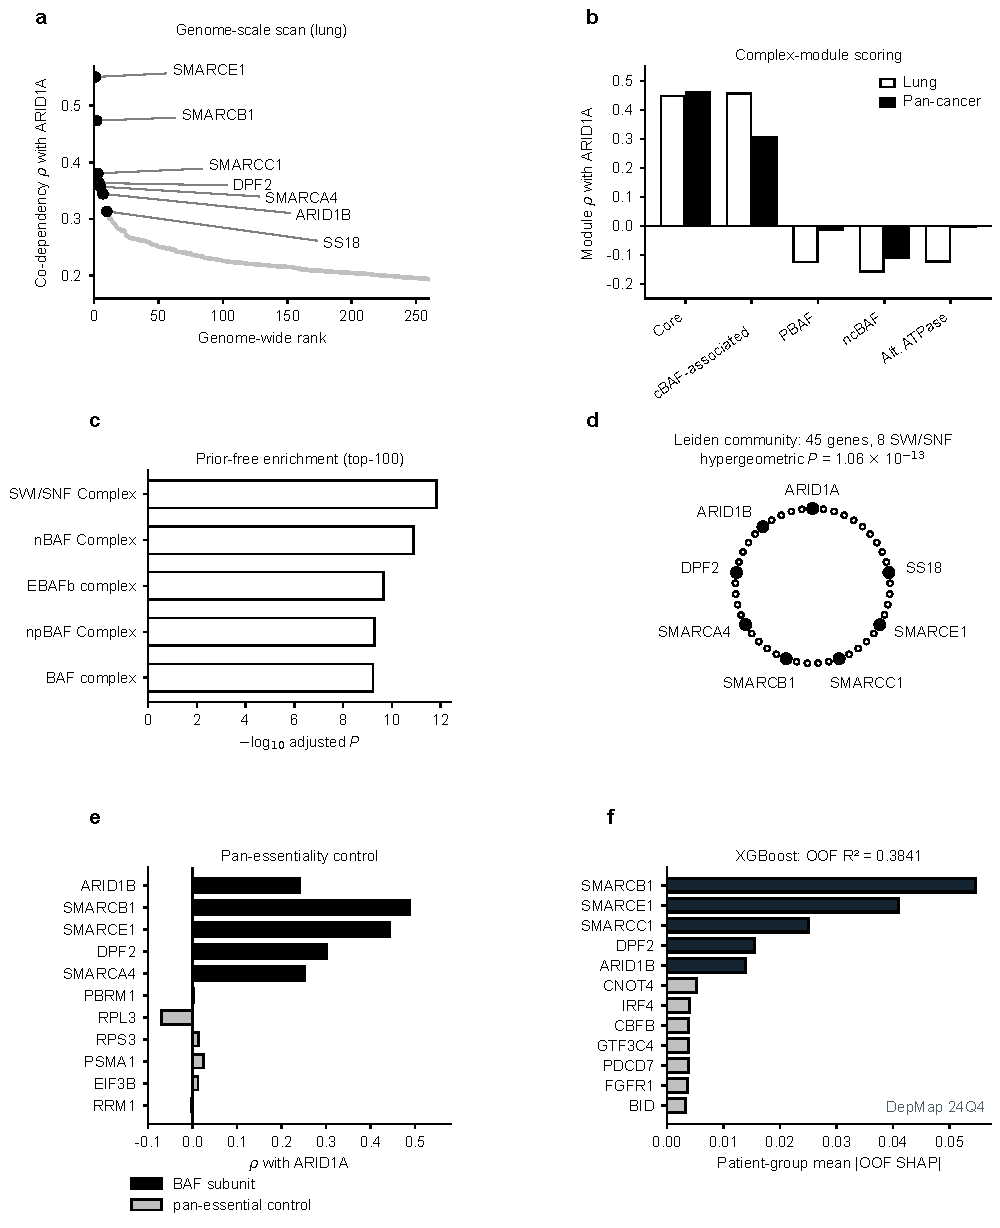
\includegraphics[width=\textwidth,height=0.72\textheight,keepaspectratio]{SupplementaryFigureS15.pdf}
\caption*{\textbf{Broad genome-scale analyses retained outside the focused main narrative.} Genome-wide co-dependency ranking, operational module scores, enrichment, community detection, pan-essentiality controls and patient-grouped XGBoost/SHAP attribution are shown. These panels provide context but do not constitute independent molecular validation, and model attribution is not causal.}
\end{figure}

\clearpage
\section*{Supplementary Figure S16}
\begin{figure}[H]
\centering
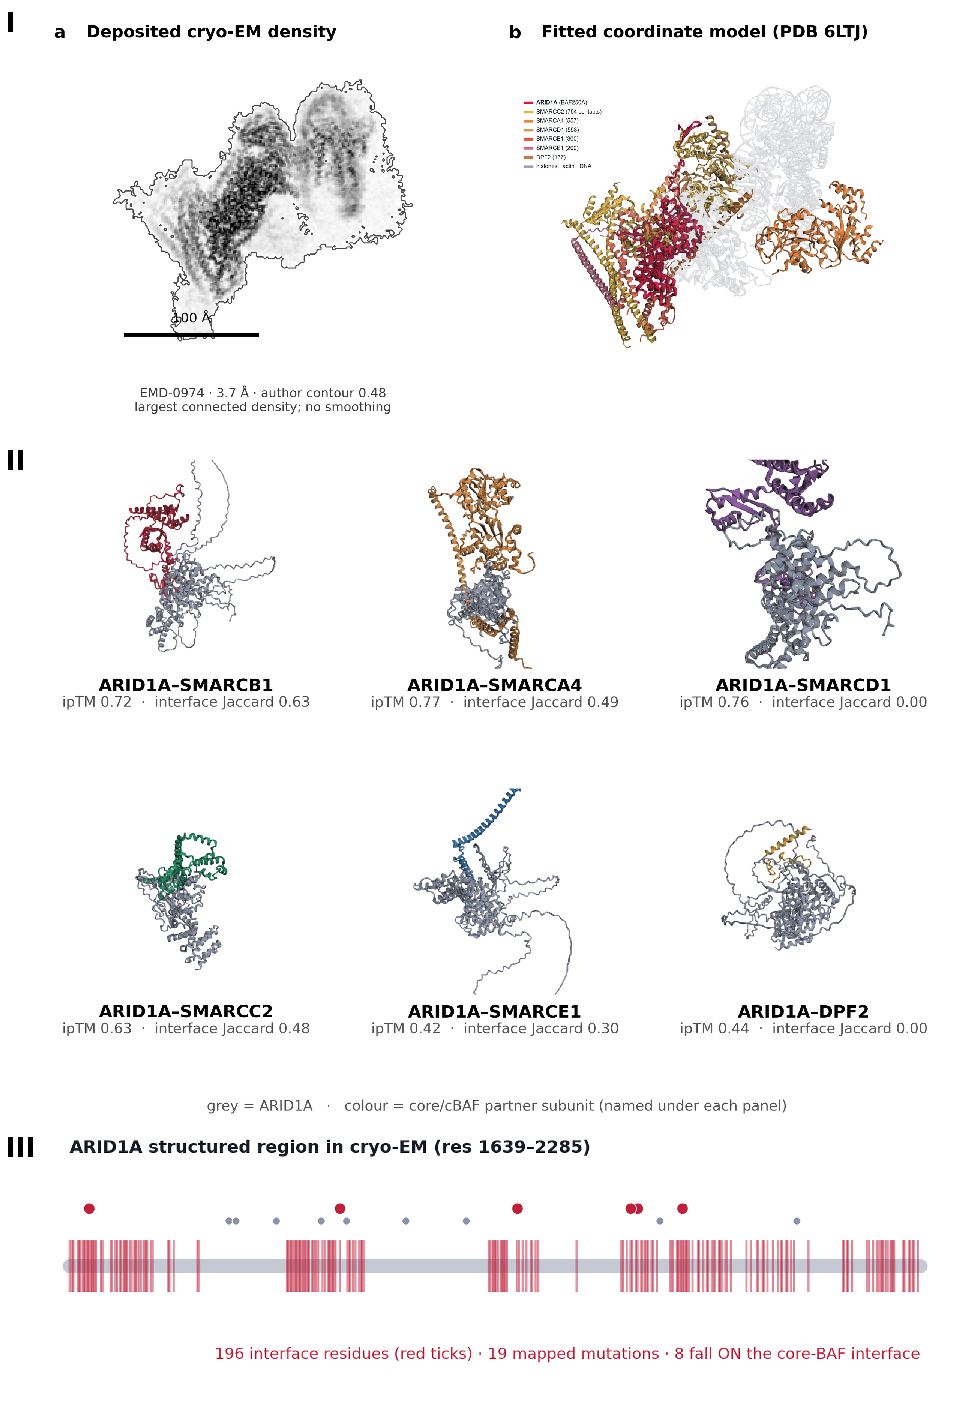
\includegraphics[width=\textwidth,height=0.72\textheight,keepaspectratio]{SupplementaryFigureS16.pdf}
\caption*{\textbf{Extended experimental, predicted and mutation-mapped structural context.} Deposited EMD-0974 density and PDB 6LTJ coordinates are shown alongside six frozen AlphaFold-Multimer models and ARID1A interface-residue mutation mapping. Predicted interfaces are exploratory and do not replace deposited experimental contacts or validate a perturbation phenotype.}
\end{figure}

\clearpage
\section*{Supplementary Figure S17}
\begin{figure}[H]
\centering
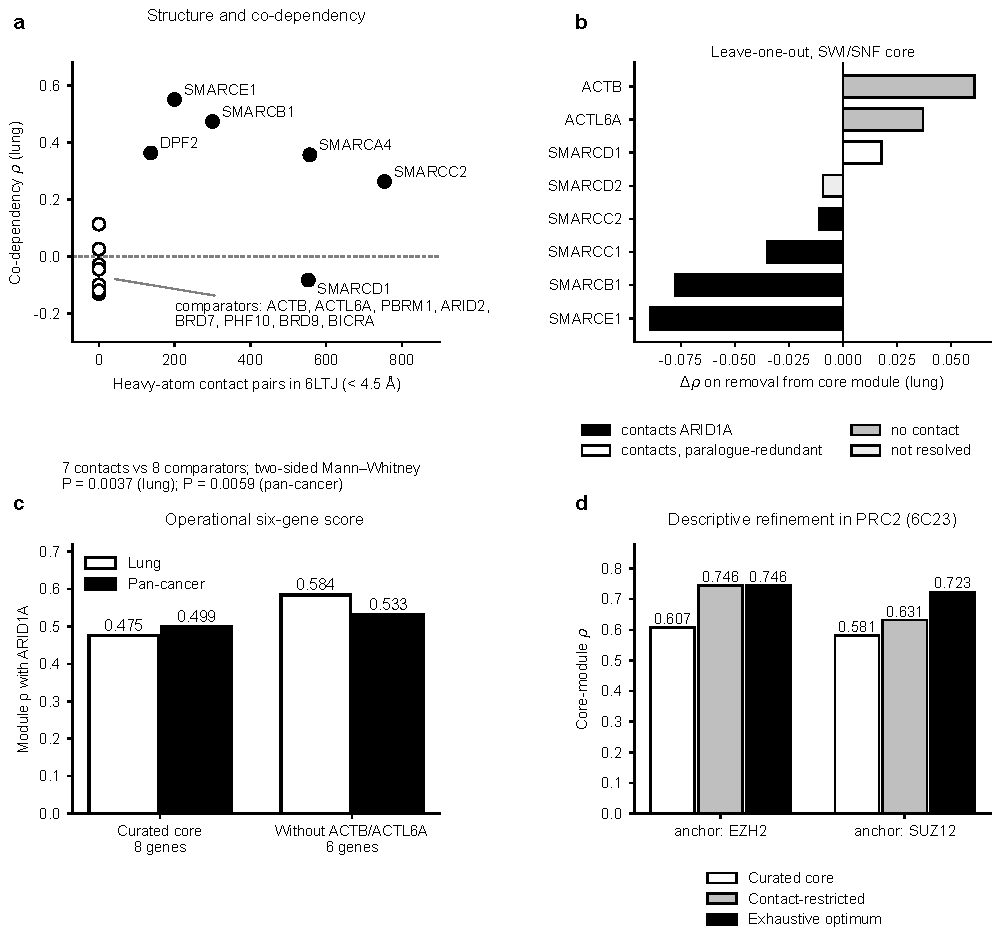
\includegraphics[width=\textwidth,height=0.72\textheight,keepaspectratio]{SupplementaryFigureS17.pdf}
\caption*{\textbf{Extended structural and score-refinement analyses.} Heavy-atom contacts are compared with co-dependency, and leave-one-out operational scores are shown for BAF and descriptive PRC2 examples. Contact, complex membership and score contribution are not interchangeable; these analyses do not define a universal member-removal rule.}
\end{figure}

\clearpage
\section*{Supplementary Figure S18}
\begin{figure}[H]
\centering
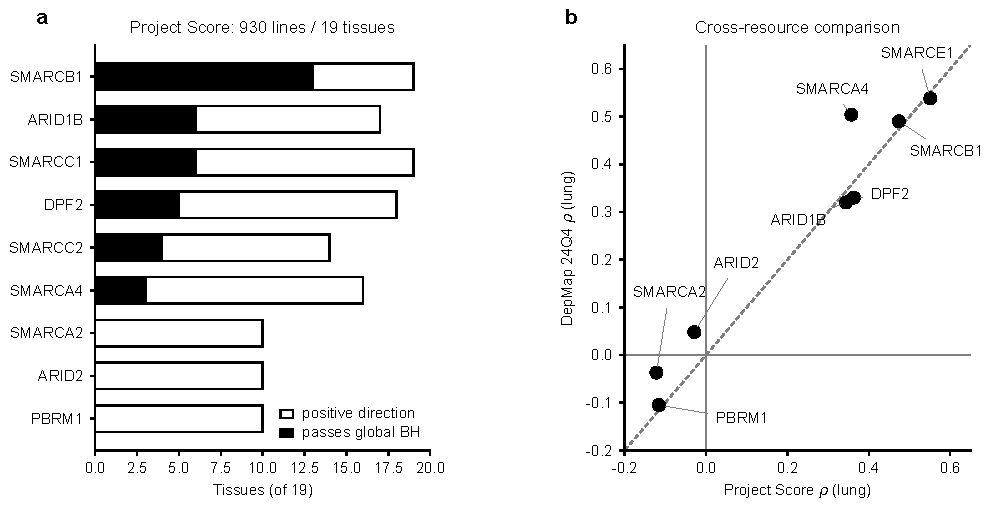
\includegraphics[width=\textwidth,height=0.72\textheight,keepaspectratio]{SupplementaryFigureS18.pdf}
\caption*{\textbf{Within-tissue and cross-release co-dependency robustness.} Within-tissue directions across 19 tissues and Project Score versus DepMap 24Q4 estimates are shown. Shared models and related screening resources make this a robustness analysis rather than independent biological replication.}
\end{figure}

\clearpage
\section*{Supplementary Figure S19}
\begin{figure}[H]
\centering
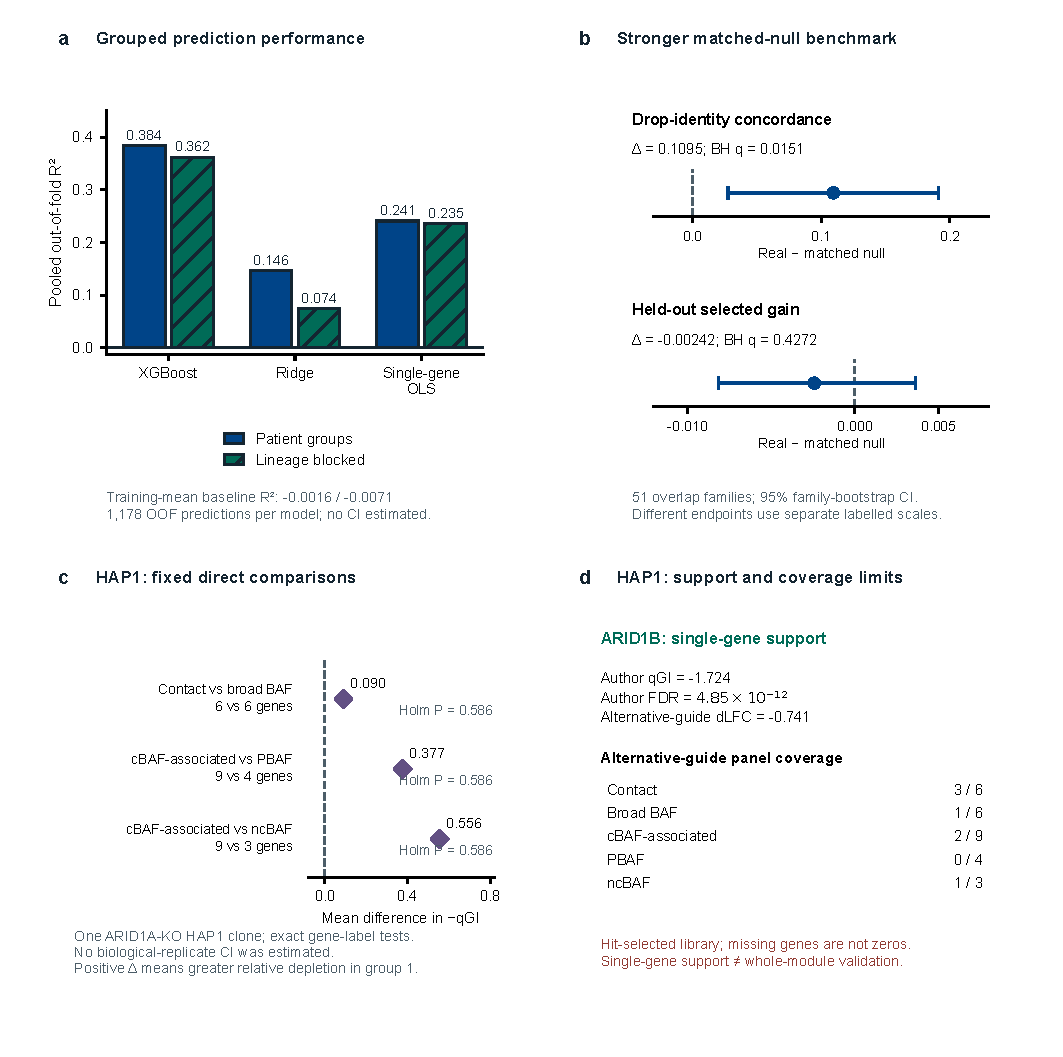
\includegraphics[width=\textwidth,height=0.72\textheight,keepaspectratio]{SupplementaryFigureS19.pdf}
\caption*{\textbf{Grouped prediction, matched cross-complex controls and HAP1 boundary analyses.} Patient- and lineage-grouped prediction, matched-null member-removal analyses and complete-panel HAP1 contrasts are retained as exploratory context. The HAP1 resource reproduces ARID1B but not a whole contact or cBAF module; statistical prediction and stable feature nomination do not establish biological dependence.}
\end{figure}

\clearpage
\section*{Supplementary Figure S20}
\begin{figure}[H]
\centering
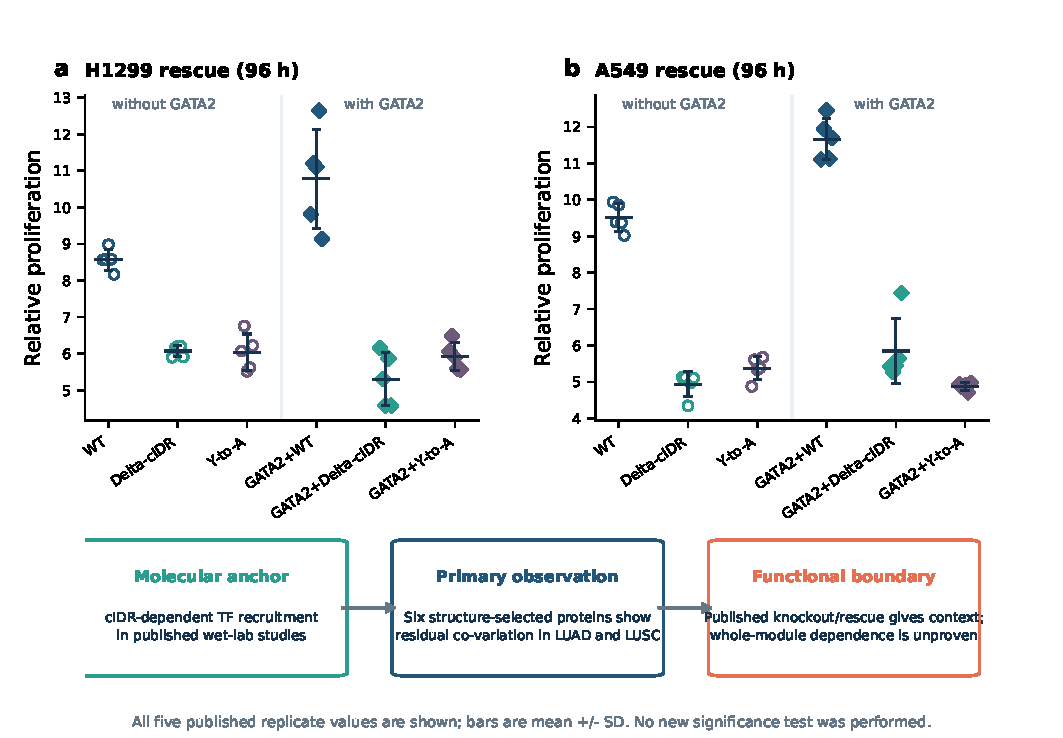
\includegraphics[width=\textwidth,height=0.72\textheight,keepaspectratio]{SupplementaryFigureS20.pdf}
\caption*{\textbf{Published ARID1A IDR-rescue data provide molecular context but not validation of the proteogenomic endpoint.} (\textbf{a},\textbf{b}) Descriptive 96-hour measurements from the openly supplied source data of Ye et al. in H1299 and A549 ARID1A-knockout cells \citep{ye2026}. Points are five deposited observations; bars show mean and standard deviation. Full-length ARID1A is compared with an IDR-deletion construct ($\Delta$cIDR) and a tyrosine-to-alanine IDR mutant, with or without GATA2. No new inferential test was performed. (\textbf{c}) These published experiments address IDR-dependent condensation and transcription-factor recruitment; they do not test whether direct ARID1A contact causes the residual protein co-variation reported in the present study.}
\end{figure}

\clearpage
\bibliographystyle{achemso}\bibliography{references_jpr}
\end{document}
